
% \setchapterpreamble[ur]{%
% \dictum[T.~Plehn~\cite{plehn_defense}]{%
% Did you know that in my PhD defence, I didn't answer a single question correctly?}%
% \vspace*{2cm}}



%%%%%%%%%%%%%%%%%%%%%%%%%%%%%%%%%%%%%%%%%%%%%%%%%%%%%%%%%%%%
\chapter{Appendices}
%%%%%%%%%%%%%%%%%%%%%%%%%%%%%%%%%%%%%%%%%%%%%%%%%%%%%%%%%%%%

Here we collect additional examples, results, and technical details
that are not too interesting on their own, but should be included for
completeness and reproducibility. We begin with our conventions for
the Standard Model. \autoref{sec:appendix_eft_fundamentals} provides
explicit examples for the manipulation of effective Lagrangians with
field redefinitions and matching with functional methods. In
\autoref{sec:appendix_silh} we define an alternative basis for
dimension-six operators and link it to the HISZ basis used in this
thesis. Appendix~\ref{sec:appendix_models} contains some additional
details on the models considered in
\autoref{chapter:validity}. Finally, in
Appendix~\ref{sec:appendix_information} we collect some auxiliary
results related to \autoref{chapter:information}.

Large parts of this appendix has been published previously, as part of
the same articles that contained much of the main body of this
thesis. In particular, Appendices~\ref{sec:appendix_silh} and
\ref{sec:appendix_models} were part of
References~\cite{Brehmer:2015rna, Biekotter:2016ecg}, while
Appendix~\ref{sec:appendix_information} contains material published in
Reference~\cite{Brehmer:2016nyr}.



%%%%%%%%%%%%%%%%%%%%%%%%%%%%%%%%%%%%%%%%%%%%%%%%%%%%%%%%%%%%
\section{Standard model conventions}
\label{sec:appendix_sm}
%%%%%%%%%%%%%%%%%%%%%%%%%%%%%%%%%%%%%%%%%%%%%%%%%%%%%%%%%%%%

\begin{table}
  \begin{tabular}{l ccc ccc}
    \toprule
    %
    \multirow{2}{*}{Fermions} & & & & \multicolumn{3}{c}{Representation} \\
    %
    & & & & $SU(3)_C$ & $SU(2)_L$ & $U(1)_Y$ \\
    %
    \midrule
    %
    LH quarks & ${\twovec u d}_L$ & ${\twovec c s}_L$ & ${\twovec t b}_L$ & $\mathbf{3}$ & $\mathbf{2}$ & $\phantom{-} \dfrac 1 6$\\[3mm]
    RH up-type quarks & $u_R$ & $c_R$ & $t_R$ & $\mathbf{3}$ & $\mathbf{1}$ & $\phantom{-} \dfrac 2 3$ \\[3mm]
    RH down-type quarks & $d_R$ & $s_R$ & $b_R$ & $\mathbf{3}$ & $\mathbf{1}$ & $- \dfrac 1 3$ \\[3mm]
    LH leptons & ${\twovec {\nu_e} {e^-}}_L$ & ${\twovec {\nu_\mu} {\mu^-}}_L$ & ${\twovec {\nu_\tau} {\tau^-}}_L$ & $\mathbf{1}$ & $\mathbf{2}$ & $- \dfrac 1 2$ \\[3mm]
    RH leptons & $e^-_R$ & $\mu^-_R$ & $\tau^-_R$ & $\mathbf{1}$ & $\mathbf{1}$ & $- 1$ \\
    %
    \bottomrule
  \end{tabular}
  \caption{SM fermions and their representation under the SM gauge group.}
  \label{tbl:appendix_bases_fermions}
\end{table}

We begin with our conventions for the Standard Model, which also apply
to all models of new physics. The Standard Model is a renormalisable
and local quantum field theory. It is invariant under global proper
orthochronous Poincar\'e transformations (which include translations,
rotations, and boosts), and a local
$SU(3)_C \times SU(2)_L \times U(1)_Y$ gauge group. Its Lagrangian is
given by
%
\begin{align}
  \lgr{SM}
  &= - \frac 1 4 G^a_{\mu\nu} G^{a\,\mu\nu} - \frac 1 4 W^a_{\mu\nu} W^{a\,\mu \nu} - \frac 1 4 B_{\mu\nu} B^{\mu \nu}
    + \frac {\theta_{QCD}} {32 \pi^2} G^a_{\mu\nu} \widetilde{G}^{a\,\mu\nu}
    + \sum_f \overbar f \im \slashed D f \notag \\
  %
  &\phantom{=} + (D^\mu \phi)^\dagger (D_\mu \phi) - \mu^2 \phisq - \lambda (\phisq)^2 \notag \\
  %
  &\phantom{=} - \sum_{\text{generations}} \left(    y_u {\twovec {\overbar u} {\overbar d}}_L \tilde \phi \, u_{R} 
                                                           + y_d {\twovec {\overbar u} {\overbar d}}_L \phi \, d_{R}
                                                           + y_\ell {\twovec {\overbar \nu} {\overbar \ell^-}}_L \phi \, \ell_{R}  + \hc  \right ) \,.
  \label{eq:appendix_bases_sm_lagrangian}
\end{align}

The fields in this Lagrangian are a scalar $\phi$ transforming as the
$(\mathbf{1}, \mathbf{2}, 1/2)$ representation of the SM gauge group;
the gauge bosons $G_\mu^a$, $W_\mu^a$, and $B_\mu$; and the fermions
given in \autoref{tbl:appendix_bases_fermions}.  We usually leave out
generation (flavour) indices and simply denote up-type quarks,
down-type quarks, charged leptons, and neutrinos with $u$, $d$,
$\ell$, $\nu$; and the left-handed doublets with $Q$ and $L$.
\autoref{eq:appendix_bases_sm_lagrangian} includes the field strength
tensors
%
\begin{align}
  G_{\mu\nu}^a &= \partial_\mu G^a_\nu - \partial_\nu G^a_\mu + g_s f^{abc} G^b_\mu G^c_\nu \, , \\
  W_{\mu\nu}^a &= \partial_\mu W^a_\nu - \partial_\nu W^a_\mu + g \varepsilon^{abc} W^b_\mu W^c_\nu \, , \\
  B_{\mu\nu} &= \partial_\mu B_\nu - \partial_\nu B_\mu
\end{align}
%
and the dual field strength tensor
%
\begin{equation}
  \widetilde{G}^a_{\mu \nu} = \frac 1 2 \varepsilon_{\mu \nu \rho \sigma} G^{a\,\mu\nu}
\end{equation}
%
with the totally antisymmetric tensor
$\varepsilon_{\mu \nu \rho \sigma}$.  The covariant derivatives are
defined according to the gauge charges and with a conventional minus
sign in front of the gauge term, for instance
%
\begin{align}
  D_\mu \phi &= \left( \partial_\mu - \im g \frac {\sigma^a} 2 \, W^a_\mu - \im g' \frac {1} 2 \, B_\mu \right) \phi \,, \notag \\
  %
  D_\mu {\twovec u d}_L &= \left( \partial_\mu  - \im g_s \frac {\lambda^{a}} 2 G^a_\mu - \im g \frac {\sigma^a} 2 \, W^a_\mu - \im g' \frac {1} 6 \, B_\mu  \right) {\twovec u d}_L\,.
\end{align}
%
These expressions contain the structure constants $f^{abc}$ and
$\varepsilon^{abc}$ of $SU(3)$ and $SU(2)$, as well as the Pauli
matrices $\sigma^a$ and the Gell-Mann matrices $\lambda^a$.

The Standard Model has 19 free parameters. In the form of
\autoref{eq:appendix_bases_sm_lagrangian}, they are:
%
\begin{itemize}
\item the coupling constants corresponding to the three components of
  its gauge group, $g_s$, $g$, and $g'$;
\item the real parameter $\theta_{QCD}$;
\item the two real parameters $\mu^2$ and $\lambda$ of the Higgs
  potential; and
\item the Yukawa couplings $y_f$. These are unitary, complex-valued
  matrices in flavour space, and their components correspond to 13
  physical parameters.
\end{itemize}

For $\mu^2 < 0$, the potential for $\phi$ has a minimum at the
non-zero vacuum expectation value (VEV)
%
\begin{equation}
  v^2 \equiv 2 \left| \langle {\phi} \rangle \right|^2  = - \frac {\mu^2} \lambda \,.
\end{equation}
%
Using some of the gauge freedom, we can choose that the vacuum
expectation value of $\phi$ points into the lower component of the
doublet. Expanding the four physical degrees of freedom $w_a$ and $h$
around this minimum, we have
%
\begin{equation}
  \phi = \frac 1 {\sqrt{2}} \twovec  {-w_2 - \im w_1} {v + h + \im w_3} \,.
\end{equation}
%
Plugging this into \autoref{eq:appendix_bases_sm_lagrangian}, and
diagonalising the mass matrices, one sees that the gauge bosons $W^a$
and $B$ combine with the Goldstone bosons $w_a$ to the mass
eigenstates
%
\begin{align}
  W^\pm_\mu &= \frac 1 {\sqrt 2} \left ( (W_\mu^1 - \frac 1 {gv} \partial_\mu w^1)
              \pm \im (W_\mu^2 - \frac 1 {gv} \partial_\mu w^2) \right) \,, \\
  %
  Z_\mu &= c_W  (W_\mu^3 - \frac 1 {gv} \partial_\mu w^3)  - s_W B_\mu \,, \\
  %
  A_\mu &= s_W  W_\mu^3  +    c_W B_\mu
\end{align}
%
with weak mixing angle (or Weinberg angle)
%
\begin{equation}
  c_W \equiv \cos \theta_W = \frac {g} {\sqrt{ g^2 + g'^2}} \,, \qqquad
  %
  s_W \equiv \sin \theta_W = \frac {g'} {\sqrt{ g^2 + g'^2}} 
\end{equation}
%
and masses
%
\begin{equation}
  m_W = \frac {gv} 2  \, ,  \quad  m_Z = \frac {gv} {2 c_W} \, .
\end{equation}
%
The remaining degree of freedom from $\phi$ is the physical Higgs
boson $h$ with a mass
%
\begin{equation}
  m_h^2 = {-2\mu^2} = {2\lambda} v^2 \,.
\end{equation}
%
Inserting \autoref{eq:foundations_sm_phi} into the Yukawa
couplings also yields fermion masses
%
\begin{equation}
  m_f = \frac {y_f v} {\sqrt{2}} \,.
\end{equation}
%
Since the Yukawa couplings are not flavour-diagonal, one has to
diagonalise these mass matrices in flavour space, ultimately leading
to the CKM matrix. But this does not affect the Higgs couplings, and
in this thesis we can safely assume flavour-diagonal Yukawa couplings.

With respect to the remaining gauge group $U(1)_Q$ with the gauge
boson $A_\mu$ and the gauge coupling
%
\begin{equation}
  e = \frac {g g'} {\sqrt{g^2 + g'^2}} = g s_W = g' c_W \,,
\end{equation}
%
the fermions carry the electromagnetic charge
%
\begin{equation}
  q = y + \frac {\sigma_3} 2 \,,
\end{equation}
%
where the second term is shorthand for its eigenvalue in the case of
$SU(2)_L$ doublets and zero for the singlets. More important for this
thesis, the terms that lead to mass terms for the weak gauge bosons
and fermions also yield couplings between the Higgs boson and these
particles. Expressed in terms of the masses, these couplings read
%
\begin{equation}
  g_{hff} = - \frac {m_f} v
\end{equation}
%
for the fermions and
%
\begin{equation}
  g_{hW^+ W^-} = \frac {2m_W^2} v \,, \qqqquad
  g_{hZZ} = \frac {m_Z^2} v 
\end{equation}
%
for the vector bosons.






%%%%%%%%%%%%%%%%%%%%%%%%%%%%%%%%%%%%%%%%%%%%%%%%%%%%%%%%%%%%
\section{EFT fundamentals}
\label{sec:appendix_eft_fundamentals}
%%%%%%%%%%%%%%%%%%%%%%%%%%%%%%%%%%%%%%%%%%%%%%%%%%%%%%%%%%%%



%%%%%%%%%%%%%%%%%%%%%%%%%%%%%%%%%%%%%%%%%%%%%%%%%%%%%%%%%%%%
\subsection{Nonlinear field redefinitions}
\label{sec:appendix_redefinitions}
%%%%%%%%%%%%%%%%%%%%%%%%%%%%%%%%%%%%%%%%%%%%%%%%%%%%%%%%%%%%

In \autoref{sec:foundations_eft_bottom_up} we argued that non-linear
field redefinitions of the form given in
\autoref{eq:foundation_field_redefinitions_ansatz} leave the
$S$-matrix elements and thus all observable physics invariant, but
change the form of the Lagrangian. According to
\autoref{eq:foundations_field_redefinitions}, the leading term of the
change of the Lagrangian is just given by the classical equations of
motion. This defines an equivalence relation between some operators
that can be used to remove redundant operators and define a minimal
basis, as discussed in \autoref{sec:foundations_heft_operators} for
the Higgs EFT.

Here we illustrate this procedure by explicitly calculating the effect
of such a non-linear field redefinition without truncating the
Lagrangian at the leading order. We start with the $CP$-even
$B$-$\phi$ sector of the SM effective field theory, and add effective
operators up to mass dimension six. Ordering the terms by mass
dimension, it reads
%
\begin{align}
  \lgr{before}
  &= - \mu^2 \phisq \notag \\
  %
  &\phantom{=}
    - \frac 1 4 \, B_{\mu\nu} B^{\mu \nu} + (D^\mu \phi)^\dagger (D_\mu \phi) - \lambda \, (\phisq)^2 \notag \\
  %
  &\phantom{=}
    + \frac {f_{\phi,1}} {\Lambda^2} \, (D_\mu\phi)^\dagger \phi \; \phi^\dagger D^\mu\phi 
    + \frac {f_{\phi,2}} {\Lambda^2} \, \frac{1}{2}\partial^\mu(\phisq)\,\partial_\mu(\phisq)
    + \frac {f_{\phi,3}} {\Lambda^2} \, \frac{1}{3}(\phisq)^3 \notag \\
  %
  &\phantom{=}
    + \frac {f_{\phi,4}} {\Lambda^2} \, (\phisq)  (D_\mu \phi)^\dagger D^\mu \phi
    + \frac {f_{B}} {\Lambda^2} \, \frac{\im g'}{2 }(D^\mu\phi^\dagger)(D^\nu\phi)\,B_{\mu\nu}
    - \frac {f_{BB}} {\Lambda^2} \, \frac{g'^2}{4} (\phisq)\,B_{\mu\nu}\,B^{\mu\nu} \notag \\
  %
  &\phantom{=}
  + \ord{1/\Lambda^4} \,.
\end{align}

The simplest non-linear field transformation is
%
\begin{equation}
  \phi \to \phi + \frac {\varepsilon} {\Lambda^2} (\phisq) \phi \,.
  \label{eq:appendix_redefinition_ansatz_phi}
\end{equation}
%
It transforms this Lagrangian into
%
\begin{equation}
  \lgr{after} = \lgr{before} + \delta \lgr{$4$} + \delta \lgr{$6$} + \delta \lgr{$8$} + \delta \lgr{$\geq 10$}
\end{equation}
%
where the indices denote the mass dimension of the operators. The SM
dimension-two term generates
%
\begin{equation}
  \delta \lgr{$4$} = -  2 \mu^2 \, \frac {\varepsilon}{\Lambda^2} \, (\phisq)^2 \,. 
    \label{eq:appendix_redefinition_dim4}
\end{equation}
%
At the dimension-six level, we have
%
\begin{equation}
  \delta \lgr{$6$}
  =
  \frac {\varepsilon}{\Lambda^2} \left[
    \partial^\mu(\phisq) \, \partial_\mu(\phisq) 
    - 4 \lambda \, (\phisq)^3 
    + 2 \, \phisq \,  (D_\mu \phi)^\dagger \, D^\mu \phi
    \right]
    - \mu^2 \, \frac {\varepsilon^2}{\Lambda^4} \,  (\phisq)^3 \,. 
    \label{eq:appendix_redefinition_dim6}
\end{equation}
%
The effects at dimension eight read
%
\begin{align}
  \delta \lgr{$8$} &= \frac {\varepsilon}{\Lambda^4} \Biggl[
                     \frac  {\im g' f_B} {2} \; \partial_\mu (\phisq) \, (\phi^\dagger \overleftrightarrow{D}_\nu \phi) \, B^{\mu\nu}
                     + f_{\phi,4} \; \phisq \, \partial^\mu(\phisq) \, \partial_\mu(\phisq) \notag \\
  %
  &\phantom{= \frac {\varepsilon}{\Lambda^4} \Biggl[ }
                     + \im g' f_B \; \phisq \, (D_\mu\phi^\dagger) D_\nu\phi \, B^{\mu\nu} 
    + 4 f_{\phi,1} \; \phisq \, (D_\mu\phi)^\dagger \phi \, \phi^\dagger D^\mu\phi \notag \\
  %
  &\phantom{= \frac {\varepsilon}{\Lambda^4} \Biggl[ }
    + f_{\phi,1} \; \phisq \, \partial^\mu(\phisq) \, \partial_\mu(\phisq) 
    + 4 f_{\phi,4} \; (\phisq)^2 \,  (D_\mu\phi)^\dagger \, D^\mu \phi \notag \\
  %
  &\phantom{= \frac {\varepsilon}{\Lambda^4} \Biggl[ }
    - \frac 1 2 g'^2 f_{BB} \; (\phisq)^2 \, B_{\mu\nu} \, B^{\mu\nu}
    + 2 f_{\phi,3} (\phisq)^4
    \Biggr] \notag \\
  %
  &\phantom{={}}
    +\frac {\varepsilon^2}{\Lambda^4} \Biggl[
    + 2 \; \phisq \, \partial^\mu(\phisq) \, \partial_\mu(\phisq) 
    - 6 \lambda \, (\phisq)^4
    + (\phisq)^2 \,  (D_\mu \phi)^\dagger \, D^\mu \phi
    \Biggr] \,,
    \label{eq:appendix_redefinition_dim8}
\end{align}
%
and so on for higher mass dimensions.

Setting the $\ord{\varepsilon}$ terms in
Equations~\eqref{eq:appendix_redefinition_dim4} to
\eqref{eq:appendix_redefinition_dim8} to zero corresponds exactly to
the classical equations of motion for $\phi$, as discussed in
\autoref{sec:foundations_eft_bottom_up} and applied to the SM EFT in
\autoref{eq:foundations_equivalence_from_eom_phi}. The higher orders
in $\varepsilon$ are missing in the equations of motion, but including
them does not affect our choice of redundant operators.

Similarly, a transformation 
%
\begin{equation}
  B_\mu \to B_\mu + \frac {\varepsilon} {\Lambda^2} \, \phisq \, B_\mu
  \label{eq:appendix_redefinition_ansatz_b}
\end{equation}
%
will correspond to the classical equations of motion for $B_\mu$ plus
$\ord{\varepsilon^2}$ corrections.

If we use transformations like
\autoref{eq:appendix_redefinition_ansatz_phi} or
\autoref{eq:appendix_redefinition_ansatz_b} (or, equivalently, the
equations of motion) to remove redundant dimension-six operators from
the Lagrangian, we cannot use exactly the same freedom to also
manipulate dimension-eight operators in a specific way. To do so, we
have to add additional degrees of freedom to our transformations, for
instance with
%
\begin{equation}
  \phi \to \phi
  + \frac {\varepsilon} {\Lambda^2} (\phisq) \phi 
  + \frac {\varepsilon_1} {\Lambda^4} \, B_{\mu\nu} B^{\mu \nu} \, \phi 
  + \frac {\varepsilon_2} {\Lambda^4} \, (D^\mu \phi)^\dagger (D_\mu \phi)  \, \phi
  + \frac {\varepsilon_3} {\Lambda^4}  \, (\phisq)^2 \, \phi  \,.
\end{equation}
%
The new parameters $\varepsilon_i$ will generate dimension-six
operators from the $\mu^2$ term and dimension-eight operators from the
SM dimension-four terms. Again, the $\ord{\varepsilon_i}$ terms in the
transformed Lagrangian correspond to the equations of motion in
$\phi$, now multiplied with dimension-four operators. Combined
transformations as in \autoref{eq:appendix_redefinition_ansatz_phi}
let us remove redundant dimension-six and dimension-eight operators
simultaneously. 





%%%%%%%%%%%%%%%%%%%%%%%%%%%%%%%%%%%%%%%%%%%%%%%%%%%%%%%%%%%%
\subsection{Functional matching}
\label{sec:appendix_functional_matching}
%%%%%%%%%%%%%%%%%%%%%%%%%%%%%%%%%%%%%%%%%%%%%%%%%%%%%%%%%%%%

In \ref{sec:foundations_matching} we discussed the effective theory in
a top-down approach, finally arriving at the expression for the
effective action at one-loop level given in
\autoref{eq:effective_action_result}.

We now show how this object can be calculated with functional methods
in a simple example.  We consider a theory of two real scalar
fields. The light field $\phi$ has mass $m$, the heavy field $\Phi$
with mass $M$ is being integrated out. The underlying theory is given
by
%
\begin{multline}
  S[\phi,\Phi] = \intfourx \Biggl[
    \frac 1 2 \partial_\mu \phi \partial^\mu \phi
    - \frac {m^2} 2 \phi^2
    + \frac 1 2 \partial_\mu \Phi \partial^\mu \Phi
    - \frac {M^2} 2 \Phi^2 \\
    - \frac {\lambda_0} {4!} \phi^4
    - \frac {\lambda_2} {4} \phi^2 \Phi^2
    - \frac {\lambda_4} {4!} \Phi^4
    \Biggr] \,.
\end{multline}
%
Odd interactions and a mixing term $\phi\Phi$  are forbidden with suitable $\mathbb{Z}_2$
symmetries.

The classical equation of motion for $\Phi$ is
%
\begin{equation}
  \left( \partial^2 + M^2 + \frac {\lambda_2} 2 \phi^2 + \frac {\lambda_4} {3!} \Phi_c^2 \right) \Phi_c = 0
\end{equation}
%
with the trivial solution $\Phi_c = 0$.

The first term in the effective action then just gives back $\phi^4$
theory for the light field, without any new effective interactions:
%
\begin{equation}
  S[\phi,\Phi_c] = \intfourx \left[\frac 1 2 \partial_\mu \phi \partial^\mu \phi - \frac {m^2} 2 \phi^2 - \frac {\lambda_0} {4!} \phi^4 \right] \,.
  \label{eq:foundations_scalar_example_effective_action_tree_part}
\end{equation}
%
The second term is
%
\begin{align}
  \frac \im 2 \tr \log \left( - \left. \frac {\delta^2 S} {\delta \Phi^2} \right|_{\Phi = \Phi_c} \right) 
  %
  &=  \frac \im 2  \tr \log \left( \partial^2 + M^2 + \frac {\lambda_2} 2 \phi^2 \right) \notag \\
  %
  &=  \frac \im 2  \tr \log \left( \partial^2 + M^2 \right) + \frac \im 2  \tr \log \left( 1 + \frac {\lambda_2} 2 \frac {1} {\partial^2 + M^2 + \im \varepsilon} \phi^2 \right) \,,
  %
  % &=  \frac \im 2  \intfourk \braket {k| \log \left( \partial^2 + M^2 \right) | k} \notag \\
  % &\phantom{=} \quad + \frac \im 2  \intfourk \braket {k| \log \left( 1 + \frac {\lambda_2} 2 \frac {1} {\partial^2 + M^2 + \im \varepsilon} \phi^2 \right) | k} \,.
\end{align}
%
where derivatives in the denominator are defined as Green's
functions. Since $\tr \log \left( \partial^2 + M^2 \right) $ is just a
constant that can be calculated for instance in dimensional
regularisation, the first part does not give us any higher-dimensional
operators of the light fields $\phi$. Expanding the logarithm in the
second term, we find
%
\begin{equation}
  \seff \supset \frac {\im \lambda_2} 4  \tr \frac {1} {\partial^2 + M^2 - \im \varepsilon} \phi^2
  - \frac {\im \lambda_2^2} 8  \tr \left( \frac {1} {\partial^2 + M^2 - \im \varepsilon} \phi^2 \right)^2
  + \frac {\im \lambda_2^3} {12}  \tr \left( \frac {1} {\partial^2 + M^2 - \im \varepsilon} \phi^2\right)^3 
  + \ord{\lambda_2^4} \,.
  \label{eq:foundations_scalar_example_effective_action_powers}
\end{equation}
%
The first of these terms renormalises the $\phi$ mass term, and
the second contributes to the $\phi^4$ interaction. This is
important for RG running, but does not create the kind of new
effective interactions we are interested in here. We instead focus on
the last term and evaluate the functional trace:
%
\begin{align}
  \seff &\supset - \frac {\im \lambda_2^3} {12} \intfourk \braket {k| \left( \frac {1} {\partial^2 + M^2 - \im \varepsilon} \phi^2 \right)^3 |k} \notag \\
  %
  &\supset - \frac {\im \lambda_2^3} {12} \;
    \intfourx \!\! \intfoury \!\! \intfourz \!\!
    \intfourk \!\! \intfourp \!\! \intfourq 
    \braket {k| \frac {1} {\partial^2 + M^2 - \im \varepsilon} |x} \braket{x| \phi^2 |p}\notag \\
  &\phantom{\supset} \quad \quad
    \times \braket {p| \frac {1} {\partial^2 + M^2 - \im \varepsilon} |y} \braket{y| \phi^2 |q} 
    \braket {q| \frac {1} {\partial^2 + M^2 - \im \varepsilon} |z} \braket{z| \phi^2 |k} \,.
\end{align}
%
Here we have used the definition of the functional trace in
\autoref{eq:functional_trace} and inserted unity,
$1 = \intfourx \ket{x} \bra{x} = \intfourp \ket{p} \bra{p}$.
$\ket{k}$, $\ket{p}$, and $\ket{q}$ are eigenstates of the derivative
operator $\partial$,
i.\,e.~$\bra{k} \im \partial_\mu = \bra{k} k_\mu$, while $\ket{x}$,
$\ket{y}$, and $\ket{z}$ denote the eigenstates of local operators,
$\bra{x} \phi^2= \bra{x} \phi^2(x)$. Their inner product is
$\braket {x|k} = e^{-\im k x}$. Using these properties and shifting
the integration variables, we get
%
\begin{align}
  \seff &\supset - \frac {\im \lambda_2^3} {12} \;
          \intfourx \!\! \intfoury \!\! \intfourz \!\!
          \intfourk \!\! \intfourp \!\! \intfourq
          \frac {1} {-k^2 + M^2 - \im \varepsilon} e^{\im k x}  \phi(x)^2 e^{-\im p x} \notag \\
  &\phantom{\supset} \qquad
    \times \frac {1} {-p^2 + M^2 - \im \varepsilon} e^{\im p y}  \phi(y)^2 e^{-\im q y}  \;
    \frac {1} {-q^2 + M^2 - \im \varepsilon} e^{\im q z}  \phi(z)^2 e^{-\im k z} \notag \\
  %
  &\supset \frac {\im \lambda_2^3} {12} \;
    \intfourx \!\! \intfoury \!\! \intfourz \!\!
    \intfourk \!\! \intfourp \!\! \intfourq
    \phi(x)^2 \phi(y)^2 \phi(z)^2 \notag \\
  &\phantom{\supset} \qqquad 
    \times \frac {e^{\im p (z-x)} \, e^{\im q (z-y)}}
    { (k^2 - M^2 + \im \varepsilon) \, ((k+p)^2 - M^2 + \im \varepsilon) \,  ((k+p+q)^2 - M^2 + \im \varepsilon)} \,.
\end{align}

We can now perform the integral over the loop momentum $k$ with
Feynman parameters:
%
\begin{align}
  &\intfourk \frac {1}
              { (k^2 - M^2 + \im \varepsilon) \,
              ((k+p)^2 - M^2 + \im \varepsilon) \,
              ((k+p+q)^2 - M^2 + \im \varepsilon)} \notag \\
  %
   &\quad = 2 \int_0^1 \!\! \diff x_1 \int_0^{1-x_1} \!\! \diff x_2 \intfourk
     \Bigl[  x_1  (k^2 - M^2 + \im \varepsilon)
     + x_2 ((k+p)^2 - M^2 + \im \varepsilon) \notag \\
  &\quad \phantom{=} \qqqquad \qqquad
    + (1-x_1 -x_2)  ((k+p+q)^2 - M^2 + \im \varepsilon)  \Bigr]^{-3} \notag \\
  %
   &\quad = 2 \int_0^1 \!\! \diff x_1 \int_0^{1-x_1} \!\! \diff x_2 \intfourk
     \frac 1 { \left[ (k + a)^2 - B  + \im \varepsilon \right]^3 }
\end{align}
%
with $a = (1 - x_1) p  + (1 - x_1 - x_2) q $ and
$B = M^2 - (1 - x_1 - x_2) (p+q)^2 - x_2 p^2 + a^2$.
Shifting the loop momentum as $k \to k + a$, we finally arrive at
%
\begin{equation}
  T_3(p,q)  
   = 2 \int_0^1 \!\! \diff x_1 \int_0^{1-x_1} \!\! \diff x_2 \intfourk
     \frac 1 { \left[ k^2 - B + \im \varepsilon \right]^3 } \,.
  \label{eq:foundations_scalar_example_loop_function}
\end{equation}

To evaluate this, we first Wick-rotate $k^0 = \im k_E^0$. Formally,
this means shifting the integration path in the complex plane of $k^0$
from along the real axis to along the imaginary axis. The Cauchy
theorem assures that this does not change the value of the integral as
long as we chose the contour such that the poles are not caught
between the two contours. Defining
$k_E^2 = (k^0_E)^2 + \boldsymbol{k}^2 = - k^2$, we find
%
%\footnote{This
%  step requires $B>0$. In our case, $p$ and $q$ correspond to momenta
%  of the light fields, and in the validity regime of the EFT we should
%  always have $M^2 \gg p^2, q^2$ and therefore $B > 0$.}
%
\begin{equation}
  I_{0,3} 
   \equiv \intfourk \frac 1 { \left[ k^2 - B + \im \varepsilon \right]^3 } 
   = \im \intfourke \frac 1 { \left[ - k_E^2 - B \right]^3 } \,,
\end{equation}
%
where the $+ \im \varepsilon$ is no longer necessary. With
$\overbar{k} = |k_E |$ we can finally calculate the integral:
%
\begin{align}
  I_{0,3} = \frac {2 \pi^2} {(2 \pi)^4} \,
            \int \!\! \diff \overbar{k} {\overbar{k}}^3 \;
    \frac 1 { \left[ {\overbar{k}}^2 + B \right]^3 }
            = \frac {- \im } {32 \pi^2 B} \,.
\end{align}

Collecting all the pieces, we have
%
\begin{multline}
  \seff \supset \frac {\lambda_2^3} {192 \pi^2} \,
    \intfourx \!\! \intfoury \!\! \intfourz \phi(x)^2 \phi(y)^2 \phi(z)^2 
    \intfourp \!\! \intfourq e^{\im p (z-x)} \, e^{\im q (z-y)} \\
    \times \int_0^1 \!\! \diff x_1 \int_0^{1-x_1} \!\! \diff x_2 \;
    \left[ M^2 - (1 - x_1 - x_2) (p+q)^2 - x_2 p^2 + ((1-x_1) p  + (1 - x_1 - x_2) q )^2 \right]^{-1} \,.
\end{multline}
%
At first glance, this is disappointing: this effective action looks
non-local and involves highly non-trivial integrals. It turns out that
these can in fact be calculated and give a finite
result~\cite{tHooft:1978jhc, Denner:1991kt}. The full expression is
quite ugly, but we fortunately do not need it. Instead, we expand the
integrand in powers of $1/M^2$. We only calculate the leading term at
$\ord{1/M^2}$. Since it produces a finite result as well, the rest
term at $\ord{1/M^4}$ also has to be finite. Even more, we can argue
that the rest term at $\ord{1/M^4}$ has to vanish: the coefficient at
a given order $1/M^k$ in this expansion is an integral without any
mass scales, and has to lead to a result of mass dimension $k-2$. Only
$k = 2$ can give a non-zero and finite result, all higher orders
therefore have to vanish.\comment{Something is fishy. Check this
  argument, and check discrepancy with Denner's habil!}
% Physically, this corresponds to approximating the loop momenta
% as lighter then the heavy mass scale, which makes sense in the
% validity region of the EFT.
In this way, we find the much simpler result
%
\begin{align}
  \seff &\supset \frac {\lambda_2^3} {192 \pi^2 \,M^2 } 
    \intfourx \!\! \intfoury \!\! \intfourz 
    \phi(x)^2 \phi(y)^2 \phi(z)^2
    \intfourp \!\! \intfourq  e^{\im p (z-x)} e^{\im q (z-y)}  \notag\\
        &\phantom{\supset} \qqqquad \qqqquad \qqqquad + \ord{1/M^4} \notag \\
  %
  &\supset \frac {\lambda_2^3} {192 \pi^2 M^2 } 
    \intfourx \!\! \intfoury \!\! \intfourz
    \phi(x)^2 \phi(y)^2 \phi(z)^2 \,
    \delta (z-x) 
    \delta (z-y) \notag \\
  %
  &\supset \frac {\lambda_2^3} {192 \pi^2 M^2 } 
    \intfourx
    \phi(x)^6 \,.
    \label{eq:foundations_scalar_example_effective_action_loop_part}
\end{align}
%
After the expansion in $1/M$, we have finally arrived at a local
theory!

What about the higher terns in
\autoref{eq:foundations_scalar_example_effective_action_powers}?
Their calculation is analogous to the one presented here and leads
to operators like $\phi^8$ and higher. They are suppressed at
least with $ 1 / M^4$ and are thus irrelevant for our dimension-six
effective theory.

Collecting the pieces in
\autoref{eq:foundations_scalar_example_effective_action_tree_part}
and
\autoref{eq:foundations_scalar_example_effective_action_loop_part},
up to one loop and $\ord{1/M^2}$ the full effective action is given by
%
\begin{equation}
  \seff[\phi] = \intfourx \left[\frac 1 2 \partial_\mu \phi \partial^\mu \phi
    - \frac {m^2} 2 \phi^2 - \frac {\lambda_0} {4!} \phi^4
    + \frac {\lambda_2^3} {12 (4 \pi)^2 M^2 } \, \phi^6\right] \,.
\end{equation}
%
As expected, the dimension-six operator is suppressed by two powers of
the heavy scale $\Lambda \equiv M$, and the Wilson coefficient
consists of the couplings $\lambda_2^3$ times a loop factor.




%%%%%%%%%%%%%%%%%%%%%%%%%%%%%%%%%%%%%%%%%%%%%%%%%%%%%%%%%%%%
\section{SILH basis}
\label{sec:appendix_silh}
%%%%%%%%%%%%%%%%%%%%%%%%%%%%%%%%%%%%%%%%%%%%%%%%%%%%%%%%%%%%

For the dimension-six operators of linear Higgs effective field
theory, we nearly entirely follow the conventions of
References~\cite{Corbett:2012ja, Juan_thesis, Tyler_thesis}, which is
based on the Hagiwara-Ishihara-Szalapski-Zeppenfeld basis
(HISZ)~\cite{Hagiwara:1993ck}. Our framework is defined in
\autoref{sec:foundations_heft_operators}. The Lagrangian is given in
\autoref{eq:sm_eft}, and the operators are listed in
Tables~\ref{tbl:foundations_operators_bosonic_even} to
\ref{tbl:foundations_operators_bosonic_odd}. We discuss the
phenomenology of these operators in
\autoref{sec:foundations_heft_pheno}.

Another common basis for dimension-six operators was developed in
References~\cite{Giudice:2007fh, Contino:2013kra} and is usually names
``Strongly Interacting Light Higgs'' or ``SILH'' after the first of
these publications.  It is based on the Lagrangian
%
\begin{align}
  \lgr{SILH}
  &=
    %
    \lgr{SM}
    + \frac {c_H}{2v^2} \, \opesilh{H}
    + \frac {c_T}{2v^2} \, \opesilh{T}
    - \frac {c_6\lambda}{v^2} \opesilh{6} \notag \\
  %
  &+ \frac{\im gc_W}{2m^2_W} \, \opesilh{W}
    + \frac{\im g'c_B}{2m_W^2} \, \opesilh{B} 
    + \frac{\im g \, c_{HW}}{m_W^2} \, \opesilh{HW}
    + \frac{\im g'c_{HB}}{m_W^2} \, \opesilh{HB} \notag \\
  %
  &+ \frac{g'^2 c_\gamma}{m_W^2} \, \opesilh{\gamma}
    + \frac{g_s^2 c_g}{m_W^2} \, \opesilh{g} 
    - \sum_f \frac{c_f}{v^2} \, y_f \, \opesilh{f}
\end{align}
%
with the Wilson coefficients $c_i$ and the operators $\opesilh{i}$
defined in \autoref{tbl:appendix_bases_silh}. Note that this
Lagrangian is not of the form given in
\autoref{eq:foundations_EFT_lagrangian}: the dimension-six operators
are suppressed by powers of $m_W$ or $v$ instead of the cutoff scale
$\Lambda$.

\begin{table}
    \renewcommand{\arraystretch}{1.8}
    \begin{tabular}[t]{r @{${}={}$}l @{\hspace{0.8cm}} r @{${}={}$}l} 
      \toprule
      %
      $\opesilh{H}$ & $\partial^\mu(\phisq)\,\partial_\mu(\phisq)$ & 
      $\opesilh{HB}$ & $(D^\mu\phi^\dagger)\,(D^\nu\phi)\,B_{\mu\nu}$ \\
      %
      $\opesilh{T}$ & $(\phi^\dagger\,\overleftrightarrow{D}^\mu\,\phi)\,(\phi^\dagger\,\overleftrightarrow{D}_\mu\,\phi)$ &
      $\opesilh{HW}$ & $(D^\mu\phi^\dagger)\,\sigma^k\,(D^\nu\,\phi)\,W^k_{\mu\nu}$ \\ 
      %
      $\opesilh{6}$ & $(\phisq)^3$  &
      $\opesilh{B}$ & $(\phi^\dagger\,\overleftrightarrow{D}^\mu\,\phi)\,(\partial^\nu\,B_{\mu\nu})$ \\ 
      %
      $\opesilh{u}$ & $(\phisq)\,(\phi^\dagger\cdot\,\overbar{Q}_L)\,u_R + \hc$ &
      $\opesilh{W}$ & $\left(\phi^\dagger\,\sigma^k\,\overleftrightarrow{D}^\mu\phi\right)\,(D^\nu\,W^k_{\mu\nu})$ \\
      %
      $\opesilh{d}$ & $(\phisq)\,(\phi\, \overbar{Q}_L)\,d_R  + \hc $&
      $\opesilh{g}$ & $(\phisq)\,G^a_{\mu\nu}\,G^{\mu\nu\, a}$ \\
      %
      $\opesilh{\ell}$ & $(\phisq)\,(\phi\, \overbar{L}_L)\,l_R  + \hc $&
      $\opesilh{\gamma}$ & $(\phisq)\,B_{\mu\nu}\,B^{\mu\nu}$ \\
      %
      \bottomrule
    \end{tabular}
  \caption{Dimension-six operators in the SILH basis relevant for Higgs physics.}
  \label{tbl:appendix_bases_silh}
\end{table}

These operators can be translated to our conventions (the HISZ basis)
with the following dictionary:
%
\begingroup%
\allowdisplaybreaks%
\begin{align}
  \opesilh{H}  &= 2\ope{\phi2}\,,  &
  \opesilh{HB}  &= -\frac{2 \im }{g'}\ope{B}\,, \notag \\ 
  \opesilh{T}  &= 2\ope{\phi2}  -  4\ope{\phi1}\,,  &
  \opesilh{HW} &= -\frac{2\im }{g} \ope{W}\,,  \notag \\ 
  \opesilh{6} &= 3 \ope{\phi3} \,, & 
  \opesilh{B}  &= \frac{2 \im}{g'}  \left( \ope{BB} +  \ope{BW} - 2\ope{B} \right)\,, \notag \\ 
  \opesilh{u} &= \ope{u} \,, & 
  \opesilh{g}  &= \ope{GG} \,,  \notag \\
  \opesilh{d} &= \ope{d} \,, & 
  \opesilh{W}  &= \frac{2 \im}{g}  \left( \ope{WW} +  \ope{BW} - 2\ope{W}   \right)\,,  \notag \\ 
  \opesilh{\ell} &= \ope{\ell} \,, & 
  \opesilh{\gamma} &= -\frac{4}{g'^2}  \ope{BB}  \,.
\end{align}%
\endgroup
%
For the Wilson coefficients, we find
%
\begingroup%
\allowdisplaybreaks%
\begin{align}
  c_H &= \frac{v^2}{\Lambda^2}\,\left(\frac{1}{2}f_{\phi1}+f_{\phi2}\right)\,, &
  c_{HB} &= \frac{v^2}{\Lambda^2}\,\frac{g^2}{8} (f_{B}+2f_{BW}-2f_{WW}) \,, \notag\\
  c_T &= -\frac{v^2}{\Lambda^2}\,\frac{1}{2}f_{\phi1}\,, & 
  c_{HW} &= \frac{v^2}{\Lambda^2}\,\frac{g^2}{8} (f_{W}+2f_{WW}) \,, \notag\\
  c_6 &= -\frac{v^2}{\Lambda^2}\,\frac{1}{3\lambda}f_{\phi3}\,, &
  c_B &= \frac{v^2}{\Lambda^2}\,\frac{g^2}{4} (f_{WW}-f_{BW}) \,, \notag\\
  c_u &= - \frac{v^2}{\Lambda^2}\,\frac{1}{y_u} \, f_u \,, &
  c_W &= -\frac{v^2}{\Lambda^2}\,\frac{g^2}{4}f_{WW} \,, \notag\\
  c_d &= - \frac{v^2}{\Lambda^2}\,\frac{1}{y_d} \, f_d \,, &
  c_g &= \frac{v^2}{\Lambda^2}\,\frac{g^2}{4g_s^2}f_{GG}\,, \notag\\
  c_\ell &= - \frac{v^2}{\Lambda^2}\,\frac{1}{y_\ell} \, f_\ell \,, &
  c_\gamma &= \frac{v^2}{\Lambda^2}\,\frac{g^2}{16} (f_{BW}-f_{BB}-f_{WW}) \, .
\end{align}%
\endgroup



% %%%%%%%%%%%%%%%%%%%%%%%%%%%%%%%%%%%%%%%%%%%%%%%%%%%%%%%%%%%%
% \subsection{Other operators}
% %%%%%%%%%%%%%%%%%%%%%%%%%%%%%%%%%%%%%%%%%%%%%%%%%%%%%%%%%%%%

% As we discussed in \autoref{sec:foundations_heft_operators}, effective
% operators can be manipulated and replaced by others without changing
% the physics through field redefinitions, integration by parts, and a
% numnber of identities. Here we demonstrate how these relations can be
% used to translate the operators
% %
% \begin{align}
%   \opeother{r} &= \phisq\, (D_\mu \phi)^2\,, &
%   \opeother{HF} &= \left( \bar{f}_L \, \gamma^\mu \, \sigma^a \, f_L \right) \left( \phi^\dagger \, \sigma^a \, \overleftrightarrow{D}_\mu \, \phi \right)  \,,
%   \notag \\
%   \opeother{D} &= \left( D^2 \, \phi \right)^2\,, &
%   \opeother{HH} &= \left( \phi^\dagger \, \sigma^a \, \overleftrightarrow{D}_\mu \, \phi \right)\left( \phi^\dagger \, \sigma^a \, \overleftrightarrow{D}_\mu \, \phi \right)\,.
% \end{align}
% %
% into the HISZ or SILH form. Such non-standard operators can arise in
% the matching procedure, see Appendix~\ref{sec:appendix_models_triplet}
% for an example.

% First, $\opeother{HH}$ can be replaced by using the completeness relation of the Pauli matrices, which for arbitrary SU(2) doublets $\xi,\,\chi,\,\eta,\,\psi$ leads to
% %
% \begin{align}
%   (\xi^\dagger \sigma^a \chi)(\eta^\dagger \sigma^a \psi)
%   &= \sum_{ijkl} \xi^*_i \sigma^a_{ij} \chi_j \, \eta^*_k \sigma^a_{kl} \psi_l \notag \\
%   %
%   &= \sum_{ijkl} (2\delta_{il}\delta_{jk}-\delta_{ij}\delta_{kl})\xi^*_i \chi_j \, \eta^*_k \psi_l \notag \\
%   %
%   &= 2(\xi^\dagger\psi)(\eta^\dagger\chi)-(\xi^\dagger \chi)(\eta^\dagger\psi)\,.
% \end{align}
% %
% Thus we find
% %
% \begin{align}
%   \opeother{HH}
%   &=
%     (\phi^\dagger\,\sigma^a\,D^\mu \phi)^2
%     +((D^\mu\phi^\dagger)\,\sigma^a\,\phi)^2
%     -2((D^\mu\phi^\dagger)\,\sigma^a\,\phi)(\phi^\dagger\,\sigma^a\,D_\mu \phi) \notag \\
%     % 
%   &= (\phi^\dagger\,D^\mu \phi)^2
%     + ((D^\mu\phi^\dagger)\,\phi)^2
%     -2\left[ 2((D^\mu\phi^\dagger)\,D^\mu \phi)(\phi^\dagger\phi)
%     - ((D^\mu\phi^\dagger)\,\phi)(\phi^\dagger\,D^\mu \phi) \right] \notag \\
%   % 
%   &= \ope{H} - 4 \ope{r} \,.
% \end{align}

% The equation of motion for the $W$ fields,
% %
% \begin{align}
% D^\nu W^a_{\mu \nu} 
% = - i g \, \phi^\dagger \dfrac {\sigma^a} {2} \overleftrightarrow{D}_\mu \phi 
%   - g \sum_f \bar{f}_L \dfrac {\sigma^a} {2} \gamma_\mu f_L  \,,
%  \label{eq:eom-w}
% \end{align}
% %
% gives rise to the identity
% %
% \begin{align}
%   \sum_f \opeother{HF} = \dfrac {2} {g} \, \ope{W} - {i} \, \ope{H} + 4 i \, \ope{r}  \,.
% \end{align}

% Next, a global field redefinition $\phi \to \phi + \alpha \, (\phisq) \phi / v^2$ generates a shift in the Wilson coefficients
% %
% \begin{equation}
%  c_H \to c_H + 2\alpha\,, \quad
%  c_r \to c_r + 2\alpha\,, \quad
%  c_6 \to c_6 + 4\alpha\,, \quad
%  c_f \to c_f + \alpha\,,
% \end{equation}
% %
% so with the choice
% $\alpha=-c_r/2$ one can eliminate the operator
% $\ope{r}$ in favour of other operators:
% %
% \begin{equation}
%   \opeother{r} \leftrightarrow \biggl\{ - \dfrac 1 2 \, \ope{H} + 2 \, \lambda \, \ope{6} + \sum_f \left[ \dfrac 1 2 \, y_f \, \ope{f} + \text{h.c.}\right] \biggr\} \,.
% \end{equation}

% Finally, $\ope{D}$ can be exchanged for others using the equation of
% motion for $\phi$,
% %
% \begin{equation}
%   D^2 \phi = - \mu^2  \, \phi - 2\, \lambda \, \phisq \, \phi - \sum_\text{gen.} \left[y_u \, \bar{Q}^T_L \, u_R + y_d \, \bar{d}_R \, Q_L + y_\ell \, \bar{\ell}_R \, L_L \right] \,. 
% \end{equation}
% %
% This leads to
% %
% \begin{equation}
%   \opeother{D} = \mu^4 \, \phisq 
%  + 4 \, \lambda \, \mu^2 \, (\phisq)^2 
%  + \mu^2 \, \sum_f y_f \, \bar{f}_L \phi f_R  \
%  + 4 \, \lambda^2 \, (\phisq)^3 + 2 \, \lambda \, \sum_f y_f \, \phisq \, \left( \bar{f}_L \phi f_R \right) \,.
% \end{equation}
% %
% The first three terms lead to a renormalization of the SM parameters
% $\mu$, $\lambda$, $y_f$, without any impact on physical
% observables. The last two terms, however, means that $\ope{D}$ is
% equivalent to the combination
% %
% \begin{equation}
%   \opeother{D} \leftrightarrow 4 \, \lambda^2 \, \ope{6} + 2 \, \lambda \, \sum_f \left( y_f \, \ope{f} + \text{h.c.} \right)\,.
% \end{equation}





% %%%%%%%%%%%%%%%%%%%%%%%%%%%%%%%%%%%%%%%%%%%%%%%%%%%%%%%%%%%%
% \subsection{HLM basis}
% %%%%%%%%%%%%%%%%%%%%%%%%%%%%%%%%%%%%%%%%%%%%%%%%%%%%%%%%%%%%

% Aside from the relatively simple case of the multi-Higgs sector
% extensions, we make use of the covariant derivative
% expansion~\cite{Gaillard:1985uh,Cheyette:1987qz} to analytically carry out
% the matching between the different UV completions to
% their corresponding EFT description.  The method has been recently
% reappraised in Reference~\cite{Henning:2014wua} and employed in a number of
% studies~\cite{heft_limitations,heft_limitations2,Chiang:2015ura,Huo:2015exa}.
% By applying this method, the Wilson coefficients are readily obtained
% in a different operator basis (henceforth dubbed HLM),
% %
% \begin{align}
%   \lgr{HLM} = \sum_i \dfrac{k_i} {\Lambda^2} \ope{i}''.
% \end{align}
% %
% The HLM operators involving Higgs fields and their interaction with
% gauge bosons are listed in Tab.~\ref{tab:ops2}.  In addition, the HLM
% basis contains a subset of operators with no direct correspondence to
% the bosonic SILH operators, which must be rewritten with the help of
% equations of motion and field redefinitions, as we discuss below.

% %-----------------------------------------------------------
% \begin{table}
%   \renewcommand{\arraystretch}{1.2}
%   \setlength{\tabcolsep}{1ex}
%   \centering
%     \begin{tabular}[t]{r @{${}={}$}l} 
%     \toprule
%     \multicolumn{2}{c}{HLM basis}  \\
%     \midrule
%     $\ope{H}''$ & $\frac{1}{2} \, \partial^\mu (\phisq) \,\partial_\mu (\phisq)$ \\ 
%     $\ope{6}''$ & $(\phisq)^3$  \\
%     $\ope{T}''$ & $\frac{1}{2} \left(\phi^\dagger \, \overleftrightarrow{D}^\mu \, \phi \right) \, \left(\phi^\dagger \, \overleftrightarrow{D}_\mu \, \phi \right)$ \\
%     $\ope{B}''$ & $\frac{i g'}{2} \left( \phi^\dagger \, \overleftrightarrow{D}^\mu \, \phi \right) \, \partial^\nu \, B_{\mu\nu}$ \\
%     $\ope{W}''$ & $\frac{i g}{2} \left(\phi^\dagger\,\sigma^k\,\overleftrightarrow{D}^\mu\phi\right)\,(D^\nu\,W^k_{\mu\nu})$ \\
%     $\ope{GG}''$ & $g_s^2 (\phisq)\,G^A_{\mu\nu}\,G^{\mu\nu\, A}$ \\ 
%     $\ope{BB}''$ & $g'^2(\phisq)\,B_{\mu\nu}\,B^{\mu\nu}$ \\
%     $\ope{WW}''$ & $g^2 (\phisq)\,W^k_{\mu\nu}\,W^{\mu\nu\, k}$ \\
%     $\ope{WB}''$ & $g g' \left(\phi^\dagger\sigma^k\phi \right)  \, B_{\mu\nu}\,W^{\mu\nu\, k}$ \\
%     \bottomrule 
%   \end{tabular}
%   \hspace{1cm}
%   \begin{tabular}[t]{r @{${}={}$}l} 
%     \toprule
%     \multicolumn{2}{c}{HISZ basis} \\
%     \midrule
%     $\ope{\phi1}'$  & $(D_\mu\phi)^\dagger\phi\,\phi^\dagger(D^\mu\phi)$ \\
%     $\ope{\phi2}'$  & $\frac{1}{2}\partial^\mu(\phi^\dagger\phi)\,\partial_\mu(\phi^\dagger\phi)$ \\ 
%     $\ope{\phi3}'$  &  $\frac{1}{3}(\phisq)^3$ \\
%     $\ope{GG}'$  &  $(\phisq)\,G^A_{\mu\nu}\,G^{\mu\nu\, A}$ \\
%     $\ope{BB}'$  &  $\phi^\dagger\,\hat{B}_{\mu\nu}\,\hat{B}^{\mu\nu}\,\phi  = -\frac{g'^2}{4}\phisq\,B_{\mu\nu}\,B^{\mu\nu}$ \\
%     $\ope{WW}'$  &  $\phi^\dagger\,\hat{W}_{\mu\nu}\,\hat{W}^{\mu\nu}\,\phi  = -\frac{g^2}{4}\phisq\,W^k_{\mu\nu}\,W^{\mu\nu\, k}$ \\
%     $\ope{BW}'$  &  $\phi^\dagger\,\hat{B}_{\mu\nu}\,\hat{W}^{\mu\nu}\,\phi  = -\frac{g\,g'}{4}(\phi^\dagger\sigma^k\phi)\,B_{\mu\nu}\,W^{\mu\nu\, k}$ \\
%     $\ope{B}'$  &  $(D^\mu\phi)^\dagger \hat{B}_{\mu\nu} (D^\nu\phi)  = i \frac{g}{2}(D^\mu\phi^\dagger)(D^\nu\phi)\,B_{\mu\nu}$ \\
%     $\ope{W}'$  &  $(D^\mu\phi)^\dagger \hat{W}_{\mu\nu} (D^\nu\phi)  = i \frac{g}{2}(D^\mu\phi^\dagger)\sigma^k( D^\nu\phi)\,W_{\mu\nu}^k$ \\
%     \bottomrule
%   \end{tabular}
%   \caption{Bosonic CP-conserving Higgs operators in the HLM basis
%     (left) and the HISZ basis (right). Here $\hat{B}_{\mu\nu}=i g'/2
%     B_{\mu\nu}$ and $\hat{W}_{\mu\nu}=i g \sigma^k/2 W_{\mu\nu}^k$.}
%   \label{tab:ops2}
% \end{table}
% %-----------------------------------------------------------

% The operators in Tab.~\ref{tab:ops2} translate to the SILH basis via
% \begin{align}
% \begin{aligned}
%   \ope{H}'' &= \frac 1 2 \ope{H}\,, \quad &
%   \ope{6}'' &= \ope{6}\,, \quad &
%   \ope{T}'' &= \frac 1 2 \ope{T}\,, \quad &
%   \ope{B}'' &= \frac {i g'} 2 \ope{B} \,, \quad &
%   \ope{W}'' &= \frac {i g} 2 \ope{W}\,,  \\
%   \ope{GG}'' &= g_s^2 \ope{g}\,, &
%   \ope{BB}'' &= g'^2 \ope{\gamma}\,, \quad &
%   \ope{WB}'' &= 2i g' \ope{B} - 4i g' \ope{HB} - g'^2 \ope{\gamma}\,, \hspace{-10em} \\
%   \ope{WW}'' &= -2i g' \ope{B} + 2i g \ope{W} + 4i g' \ope{HB} - 4 i g \ope{HW}  + g'^2 \ope{\gamma}  \, . \hspace{-20em}
% \end{aligned}
% \end{align}
% %
% In addition, the HLM basis contains extra operators with no SILH counterpart, 
% %
% \begin{align}
%   \ope{R}'' = \phisq \left(D_\mu \, \phi\right)^\dagger \left(D^\mu \, \phi \right)\,, \qqquad
%   \ope{D}'' = \left( D^2 \phi \right)^2 \, ,
%   \label{eq:HLM_add_ops}
% \end{align}
% %
% which can be eliminated using \autoref{eq:EFT_Or_replacement}
% and \autoref{eq:EFT_OD_replacement}, respectively.  The Wilson
% coefficients $k_i$ of the HLM basis translate to the SILH coefficients
% $\bar{c}_i$ as follows:
% %
% \begin{align}
%   \bar{c}_H &= \dfrac {v^2} {\Lambda^2} \, \left( k_H - k_R \right) \,, &
%   \bar{c}_B &= \dfrac {v^2} {\Lambda^2} \, \dfrac {g^2} 4 \, \left(k_B + 4 \, k_{WB} - 4 \, k_{WW} \right) \notag \,, \\
%   \bar{c}_T &= \dfrac {v^2} {\Lambda^2} \, k_T \,, & 
%   \bar{c}_W &= \dfrac {v^2} {\Lambda^2} \, \dfrac {g^2} 4 \, \left(k_W + 4  \, k_{WW} \right) \notag \,, \\
%   \bar{c}_6 &= - \dfrac {v^2} {\Lambda^2} \, \left( \dfrac {k_6} {\lambda} + 2\, k_R + 4 \, \lambda \, k_D \right) \,, & 
%   \bar{c}_{HB} &= \dfrac {v^2} {\Lambda^2} \, g^2 \, \left(  k_{WW} - k_{WB} \right) \notag \,, \\
%   \bar{c}_g &= \dfrac {v^2} {\Lambda^2} \, \dfrac {g^2} 4 \, k_{GG} \,,  &   
%   \bar{c}_{HW} &= - \dfrac {v^2} {\Lambda^2} \, g^2 \, k_{WW} \notag \,, \\
%   \bar{c}_\gamma &= \dfrac {v^2} {\Lambda^2} \, \dfrac {g^2} 4 \, \left( k_{BB} - k_{WB} + k_{WW} \right) \,, &
%   \bar{c}_f &= - \dfrac {v^2} {\Lambda^2} \, \left( \dfrac 1 2 \, k_R + 2 \, \lambda \, k_D \right) \,,
% \end{align}
% %
% where for the sake of completeness we have included the coefficients
% of the redundant operators given in \autoref{eq:HLM_add_ops}.







%%%%%%%%%%%%%%%%%%%%%%%%%%%%%%%%%%%%%%%%%%%%%%%%%%%%%%%%%%%%
\section{Model fine print}
\label{sec:appendix_models}
%%%%%%%%%%%%%%%%%%%%%%%%%%%%%%%%%%%%%%%%%%%%%%%%%%%%%%%%%%%%


%%%%%%%%%%%%%%%%%%%%%%%%%%%%%%%%%%%%%%%%%%%%%%%%%%%%%%%%%%%%
\subsection{Singlet extension}
\label{sec:appendix_models_singlet}
%%%%%%%%%%%%%%%%%%%%%%%%%%%%%%%%%%%%%%%%%%%%%%%%%%%%%%%%%%%%

The singlet model is defined in
Equations~\eqref{eq:validity_singlet_lagrangian} and
\eqref{eq:validity_singlet_potential} in
\autoref{sec:validity_singlet}. Ignoring the Goldstones, the
scalar doublet and singlets fields can be expanded into components as
%
\begin{align}
  \phi &= \frac{1}{\sqrt{2}} \twovec {1} {v + \phi^0} \,, \notag \\
  S &= \frac{1} {\sqrt{2}} (v_s + s^0) \,,
\end{align}
%
where $v \equiv \sqrt{2}\langle \phi \rangle = 246$~GeV and
$v_s \equiv \sqrt{2}\langle S \rangle$ denote their respective
VEVs. The minimisation condition for this potential can be used to
eliminate the parameters $\mu_{1,2}$ in favour of $v$ and
$v_s$. $\phi^0$ and $s^0$ mix to form a light ($h$) and a heavy ($H$)
mass eigenstate,
%
\begin{align}
  h &=\phi^0  \cos\alpha - s^0 \sin\alpha\,, \notag \\
  % 
  H &= \phi^0 \sin\alpha + s^0 \cos\alpha\,,
\end{align}
%
where
%
\begin{equation}
  \tan(2\alpha) = \frac{\lambda_3vv_s}{\lambda_2 v_s^2 - \lambda_1v^2}\,.
\end{equation}
% 
Their masses are
%
\begin{equation}
  m^2_{h,H} =
  \lambda_1\,v^2
  + \lambda_2\,v_s^2
  \mp |\lambda_1\,v^2 - \lambda_2\,v_s^2| \, \sqrt{1+\tan^2(2\alpha)}
\end{equation}
%
with $m_{H}^2 \approx 2 \lambda_2 v_s^2 \gg m_{h}^2$ in the limit
$v^2 \ll v_s^2$.

% To perform the matching to the EFT,
% we identify the UV scale $\Lambda \equiv \sqrt{2 \lambda_2} v_s \approx m_H$ for $v_s \gg v$. From the
% singlet-doublet mixing one then finds a universal coupling shift of
% the SM-like light Higgs to all other SM particles in
% \autoref{eq:shift2}, given by
% %
% \begin{alignat}{5}
%  \Delta \approx -\frac{\sin^2 \alpha}{2} \approx
%   -\dfrac{g_\text{eff}^2}{2} \,\biggl(\cfrac{v}{\Lambda} \biggr)^2 \,, \qquad
%   g_\text{eff} = \dfrac{\lambda_3}{\sqrt{2\lambda_2}} \, .
%  \label{eq:singlet-delta4}
% \end{alignat}
% %
% Integrating out the heavy Higgs boson we find
% %
% \begin{align}
%   \lgr{EFT}\supset \dfrac {\sin^2 \alpha} {2v^2} \; 
%    \partial^\mu (\phi^\dagger \phi) \partial_\mu (\phi^\dagger \phi) +
%    \ord{\Lambda^{-4}} \,.
% \label{eq:singlet-matching}
% \end{align}
% %
% We thus see that, up to dimension-6 operators the
% heavy-singlet--induced BSM effects in Higgs production and decay are
% completely captured by the operator $\ope{H}$
% (cf.\ Tab.~\ref{tab:operators}) with coefficient
% %
% \begin{align}
%   \bar{c}_H = \dfrac{\lambda_3^2}{2\lambda_2} \, \left(\dfrac {v} {\Lambda}\right)^2 + \ord {\frac{v^4}{\Lambda^4} } \,.
% \end{align}
% 

% The light Higgs couplings to fermions and gauge bosons in the singlet model 
% are universally suppressed relative to the SM. In the full model and the
% EFT, respectively, they are given by
% %
% \begin{align}
%   1 + \Delta_x =  \cos \alpha \,,
% \qqquad
%   1 + \Delta_x^\text{EFT} = 1-\dfrac{1}{2}\bar{c}_H \,.
% \end{align}

% A more complex pattern emerges for the
% self-interactions involving at least one heavy Higgs field.  We find
% %
% \begin{alignat}{5}
% g_{hhH}
% &= - \cfrac{g_\text{eff} \,(2m^2_{h} + m^2_{H})}{v_s}\,
%       \left[ 1+ g_\text{eff}\,\cfrac{v^2}{v_s^2} + \ord {
%   \frac{v^3}{v_s^3}} \right] 
% \sim \lambda_3 v_s + \ord{v} \,,
% \notag \\ 
% g_{hHH} 
% &=  \cfrac{g_\text{eff} v \,(m^2_{h} + 2 m^2_{H})}{v_s^2}\, 
%    \left[ 1- g_\text{eff} + \ord { \frac{v}{v_s}} \right] 
% \sim 2\lambda_3v \left( 1- \dfrac{\lambda_3}{2\lambda_2} \right) +
% \ord{\dfrac{v^2}{v_s}} \, ,
%  \label{eq:singlet-tripleheavy}
% \end{alignat}
% %
% in which we observe a characteristic non-decoupling behavior which
% manifests itself as a linear growth of $g_{hhH}$ with the heavy
% Higgs mass.  In the EFT, the leading self-interaction contribution enters
% via a dimension-8 operator, which is
% neglected in our dimension-6
% analysis. Therefore, the sole Wilson coefficient $\bar{c}_H = \sin^2 \alpha$ defines
% the singlet model EFT up to dimension 6.

% On the other
% hand, let us emphasize a key structural difference between the
% $\ope{H}$-induced and the UV-complete singlet model contributions to the
% Higgs self-coupling $hhh$. At variance with the latter, the effective
% operators also induces a new momentum structure into the self
% coupling, namely adding derivatives in the Lagrangian or energy
% dependent terms in the Feynman rules
% %
% \begin{align}
%  \lgr{} \supset
% &- \dfrac{m_{h}^2}{2v}\left[
%    \left(1-\dfrac{c_H v^2}{2\Lambda^2} \right) h^3
%    -\dfrac{2c_H v^2}{\Lambda^2 {m_{h}^2}} 
%     h \, \partial_\mu h \, \partial^\mu h \right] \notag \\
% &= - \dfrac{m_{h}^2} {2v} 
%     \left( 1 - \dfrac{1}{2} \bar{c}_H \right) 
%     h^3 
%    + \dfrac {g}{2 m_W} \bar{c}_H \; h \partial_\mu h \partial^\mu h 
% \label{eq:singlet-self},
% \end{align}
% %
% which means that the SM-like $h^3$ term is not only rescaled but
% also endowed with new Lorentz structures involving derivatives.  This
% kind of momentum dependence is encoded in the split into
% $g^{(1)}_{HHH}$ and $g^{(2)}_{HHH}$ in \autoref{eq:masslag}.  This
% effect does not correspond to the Higgs singlet mixing, where such a
% momentum dependence can only be generated via loop-induced heavy
% particle exchange with momentum-dependent couplings like a heavy
% fermion triangle.



%%%%%%%%%%%%%%%%%%%%%%%%%%%%%%%%%%%%%%%%%%%%%%%%%%%%%%%%%%%%
\subsection{Two-Higgs-doublet model}
\label{sec:appendix_models_2hdm}
%%%%%%%%%%%%%%%%%%%%%%%%%%%%%%%%%%%%%%%%%%%%%%%%%%%%%%%%%%%%

%%%%%%%%%%%%%%%%%%%%%%%%%%%%%%%%%%%%%%%%%%%%%%%%%%%%%%%%%%%%
\subsubsection{Model setup}
%%%%%%%%%%%%%%%%%%%%%%%%%%%%%%%%%%%%%%%%%%%%%%%%%%%%%%%%%%%%
 
We analyse the most general gauge invariant, $CP$-even theory for two
scalar fields with an additional $\mathbb{Z}_2$ symmetry, as defined
in Equation~\eqref{eq:validity_2hdm_potential} in
\autoref{sec:validity_2hdm}.  The Higgs mass-eigenstates follow
from the set of rotations
%
\begin{equation}
  \twovec {H^0} {h^0} = R(\alpha) \, \twovec {h^0_1} {h^0_2} \, ,
  \qqquad
  \twovec {w^0 }{ A^0 } = R(\beta)\,\twovec {a^0_1 }{ a^0_2 } \,,
  \qqquad
  \twovec {w^\pm }{ H^\pm } = R(\beta)\,\twovec {h^\pm_1 }{ h^\pm_2 } \,,
\end{equation}
%
with
%
\begin{equation}
  \phi_k = \twovec {h_k^+} {\dfrac{1}{\sqrt{2}} (v_k + h_k^0 + \im a_k) }
\end{equation}
%
and
%
\begin{equation}
  R(\theta) = \twomat {\cos\theta} {\sin\theta } {-\sin\theta} {\cos\theta} \,.
  \label{eq:appendix_models_2hdm_rotation}
\end{equation}

Since the two doublets contribute to giving masses to the weak gauge
bosons, custodial symmetry will impose tight constraints on the viable
mass spectrum of the model~\cite{Veltman:1976rt, Toussaint:1978zm,
  Frere:1982ma, Grimus:2007if, Hollik:1986gg, Beenakker:1988pv,
  Froggatt:1991qw, He:2001tp, Grimus:2008nb}.  Analytic relations
linking the different Higgs masses and mixing angles with the
Lagrangian parameters in \autoref{eq:validity_2hdm_potential} can be found
\eg in Appendix A of~\cite{Lopez-Val:2013yba}.  The conventions
%
\begin{equation}
  0 <\beta < \pi/2
  \quad \text{and} \quad
  0 \leq \beta-\alpha < \pi
\end{equation}
%
guarantee that the Higgs coupling to vector bosons has the same sign
in the 2HDM and in the SM.  As we will next show, the decoupling limit
implies that the light Higgs interactions approach the alignment
limit, where $\cos\beta \sim |\sin\alpha|$ and the couplings become
SM-like~\cite{Gunion:2002zf}.



%%%%%%%%%%%%%%%%%%%%%%%%%%%%%%%%%%%%%%%%%%%%%%%%%%%%%%%%%%%%
\subsubsection{Couplings}
%%%%%%%%%%%%%%%%%%%%%%%%%%%%%%%%%%%%%%%%%%%%%%%%%%%%%%%%%%%%

The tree-level coupling shifts of the light Higgs follow from these
rotations and are given in
Eqs.~\eqref{eq:validity_2hdm_higgs_vector_coupling} to
\eqref{eq:validity_2hdm_last_coupling}. The light Higgs
coupling to a charged Higgs pair reads
%
\begin{align}
   \frac {g_{h^0{H^+}{H^{-}}}}{g^\text{SM}_{hhh}}
  = \frac{1}{3 m_{h^0}^2}
  \left[ 
  \sin (\beta - \alpha) \left( 2 m_{H^\pm}^2 - m_{h^0}^2 \right)
  + \frac {\cos (\alpha + \beta)} {\sin (2\beta)}
  \left(2m_{h^0}^2 - \frac {2 m_{12}^2}{\sin \beta \cos \beta} \right)
  \right] \, ,
\end{align}
%
with $g^\text{SM}_{hhh} = -3 m_h^2/v$.

The loop-induced couplings are more involved, giving
%
\begin{align}
  1+\Delta_g
  &=
    \frac{1}{A_{gg}^\text{SM}} 
    \Bigg[\sum_{f = t,b}\,(1+\Delta_f)\,A_f(\tau_f) \Bigg] \,, \\
  %
  1+\Delta_\gamma
  &=
    \frac{1}{A_{\gamma \gamma}^\text{SM}} 
    \Biggl[ \sum_{f = t,b}\, N_C\,Q_f^2\,(1+\Delta_f)\,A_f(\tau_f)
    + Q^2_{\tau}\,(1+\Delta_\tau)\,A_{f}(\tau_\tau)
    + (1+\Delta_W)\, A_v(\tau_W) \notag \\
  %
 &\qqqqquad - {g}_{h^0 {H^+} {H^{-}}} \; \frac {m_W s_w} {e m_{H^\pm}^2} \; A_s(\tau_{H^{\pm}}) \Biggr] \,,
   \label{eq:appendix_models_2hdm_haa}
\end{align}
%
where $A_{xx}^\text{SM}$ are the corresponding contributions in the
SM. The conventional loop form factors read
%
\begin{align}
 A_s(\tau) &= -\frac{\tau}{2}\,\left[1-\tau f(\tau) \right] &&= 1/6 + \mathcal{O}(\tau^{-1}) \,, \notag \\
 A_f(\tau) &= \tau\left[1+(1-\tau)\,f(\tau) \right] &&= 2/3 + \mathcal{O}(\tau^{-1}) \,, \notag \\
 A_V(\tau) &= -\frac{1}{2}\,\left[2+3\tau+3(2\tau-\tau^2)\,f(\tau) \right] &&= -7/2 + \mathcal{O}(\tau^{-1}) \,,
\end{align}
%
where
%
\begin{equation}
 f(\tau) =
\begin{cases}
  - \frac 1 4 \left[ \log \frac{1 + \sqrt{1- \tau}} {1 - \sqrt{1 - \tau}} - i \pi \right]^2 & \quad \text{for } \tau < 1 \\
  \left[ \arcsin \frac 1 {\sqrt{\tau}} \right]^2 & \quad \text{for } \tau \geq 1 \,,
\end{cases}
\end{equation}
%
and $\tau_x = 4 m_x^2 / m_{h^0}^2$.



%%%%%%%%%%%%%%%%%%%%%%%%%%%%%%%%%%%%%%%%%%%%%%%%%%%%%%%%%%%%
\subsubsection{Matching}
%%%%%%%%%%%%%%%%%%%%%%%%%%%%%%%%%%%%%%%%%%%%%%%%%%%%%%%%%%%%

The effect of the second doublet on the phenomenology of the light
Higgs consists purely of shifted couplings $\Delta_x$. This allows us
to match the dimension-six model by setting equal the coupling shifts
from the full model, given by
Eqs.~\eqref{eq:validity_2hdm_higgs_vector_coupling} to
\eqref{eq:validity_2hdm_last_coupling} and
\eqref{eq:appendix_models_2hdm_haa}, to the corresponding couplings in
the dimension-six Lagrangian,
\autoref{eq:foundations_higgs_couplings}.

In a second step we then expand in $1/\Lambda$ and keep terms up to
$\ord{1/\Lambda^2}$, where $\Lambda$ is defined in the unbroken phase
for the default matching or as the physical mass $m_{A^0}$ in the
$v$-improved matching, as described in
\autoref{sec:validity_2hdm}.

This defines the effective model in a straightforward way. For more
details see Appendix~A.3 of Reference~\cite{Brehmer:2015rna}.



%%%%%%%%%%%%%%%%%%%%%%%%%%%%%%%%%%%%%%%%%%%%%%%%%%%%%%%%%%%%
\subsection{Scalar top partners}
\label{sec:appendix_models_stops}
%%%%%%%%%%%%%%%%%%%%%%%%%%%%%%%%%%%%%%%%%%%%%%%%%%%%%%%%%%%%

%%%%%%%%%%%%%%%%%%%%%%%%%%%%%%%%%%%%%%%%%%%%%%%%%%%%%%%%%%%%
\subsubsection{Model setup}
%%%%%%%%%%%%%%%%%%%%%%%%%%%%%%%%%%%%%%%%%%%%%%%%%%%%%%%%%%%%

The potential for the simplified scalar top-partner model consists of
three parts,
%
\begin{multline}
  \lgr{top partners} \supset
  %
  (D_{\mu} \tilde{Q})^\dagger  D^\mu \tilde{Q}
  + (D_\mu \tilde{t}_R )^* D^\mu \tilde{t}_R
  - \underbrace{M^2 \, \tilde{Q}^\dagger \tilde{Q}
  - M^2\, {\tilde{t}_R}^* \tilde{t}_R }_{\lgr{mass}} \\
  %
  - \underbrace{\kappa_{LL} \, (\phi \cdot \tilde{Q})^\dagger \, (\phi \cdot\tilde{Q})
  - \kappa_{RR} \, ({\tilde{t}_R}^*{\tilde{t}_R}) \, (\phi^\dagger\,\phi) }_{\lgr{Higgs}} 
  - \underbrace{\left[ \kappa_{LR} \, M \, {\tilde{t}_R}^*\,(\phi \cdot \tilde{Q}) + \hc \right]}_{\lgr{mixing}} \,.
  \label{eq:appendix_models_stops_lagrangian}
\end{multline}
%
We use the customary notation for the $SU(2)_L$ invariant product
$\phi \cdot \tilde{Q} \equiv \epsilon_{ab}\,\phi^a\,\tilde{Q}^b$, with
the help of the antisymmetric pseudo-tensor
$\epsilon^{ab} \equiv (i\sigma^2)^{ab}$ such that
$\epsilon^{12} = -\epsilon^{21} = 1$.

The term $\lgr{Higgs}$ gives rise to scalar partner masses
proportional to the Higgs vev, mirroring the supersymmetric $F$-term
contribution to the squark masses. By a similar token, the explicit
mass terms $\lgr{mass}$ are analogous to the squark soft-SUSY breaking
mass terms. $\lgr{mixing}$ is responsible for the mixing between the
gauge eigenstates, reminiscent of the MSSM $A$-terms.  In the absence
of an underlying supersymmetry, the Lagrangian features no equivalent
of the $D$-term contributions.

Collecting all bilinear terms from
\autoref{eq:appendix_models_stops_lagrangian}, we get
%
\begin{equation}
  \lgr{top partners} \supset
  \left(\tilde{t}_L^* \ \tilde{t}_R^* \right)
  \mathcal{M}_{\tilde{t}}
  \twovec {\tilde{t}_L} {\tilde{t}_R} \,,
\end{equation}
%
with the mass matrix $\mathcal{M}_{\tilde{t}}$ given in
\autoref{eq:validity_stops_mass}.  Assuming all parameters in
\autoref{eq:appendix_models_stops_lagrangian} to be real, $m_{ij}$ can
be diagonalised through the usual orthogonal transformation
$R(\theta_{\tilde{t}})$ given in
\autoref{eq:appendix_models_2hdm_rotation}.  This rotates the gauge
eigenstates $(\tilde{t}_L, \tilde{t}_R)$ into the mass basis
$(\tilde{t}_1,\tilde{t}_2)$,
% 
\begin{equation}
  % R(\theta_{\tilde{t}}) \, \mathcal{M}_{\tilde{t}}^2 \, R^\dagger(\theta_{\tilde{t}})
  % = \diag (m^2_{\tilde{t}_1}, m^2_{\tilde{t}_2})\,,
  % \qquad
  \twovec {\tilde{t}_1} {\tilde{t}_2}
  = R(\theta_{\tilde{t}}) \twovec {\tilde{t}_L} {\tilde{t}_R } \,.
\end{equation}
% 
The physical scalar partner masses and the mixing angle are then given
by
% 
\begin{align}
  m_{\tilde{t}_1}^2
  &= M_{LL}^2\cos^2\theta_{\tilde{t}}
    + M_{RR}^2\,\sin^2\theta_{\tilde{t}}
    + 2M_{LR}^2\,\sin\theta_{\tilde{t}}\cos\theta_{\tilde{t}} \,,\notag \\
  % 
  m_{\tilde{t}_2}^2
  &= M_{LL}^2\,\sin^2\theta_{\tilde{t}}
    + M_{RR}^2\,\cos^2\theta_{\tilde{t}}
    - 2M_{LR}^2\,\sin\theta_{\tilde{t}}\,\cos\theta_{\tilde{t}} \,,  \\
  %
  \tan(2\theta_{\tilde{t}})
  &= \frac{2M_{LR}^2}{M_{LL}^2-M_{RR}^2} \,.
\end{align}
%
As we assume the right-handed bottom partner $\tilde{b}_R$ to be heavy
and thus decoupled, the sbottom-like scalar eigenstate $\tilde{b}_L$
undergoes no mixing and can be readily identified with the physical
eigenstate. 



% %%%%%%%%%%%%%%%%%%%%%%%%%%%%%%%%%%%%%%%%%%%%%%%%%%%%%%%%%%%%
% \subsubsection{Couplings}
% %%%%%%%%%%%%%%%%%%%%%%%%%%%%%%%%%%%%%%%%%%%%%%%%%%%%%%%%%%%%

% The scalar partner couplings to the Higgs boson can be written as
% %
% \begin{align}
%   g_{h\tilde{t}_1\tilde{t}_1}/v &= \kappa_{LL}\,\cos^2\theta_{\tilde{t}} + \kappa_{RR}\,\sin^2\theta_{\tilde{t}} + \sin(2\theta_{\tilde{t}})\,\kappa_{LR} \,, \notag \\
%   g_{h\tilde{t}_2\tilde{t}_2}/v &= \kappa_{LL}\,\sin^2\theta_{\tilde{t}} + \kappa_{RR}\,\cos^2\theta_{\tilde{t}} - \sin(2\theta_{\tilde{t}})\,\kappa_{LR} \,, \notag \\
%   g_{h\tilde{b}_L\tilde{b}_L}/v & = \kappa_{LL} \,.
% \end{align}



%%%%%%%%%%%%%%%%%%%%%%%%%%%%%%%%%%%%%%%%%%%%%%%%%%%%%%%%%%%%
\subsubsection{Matching}
%%%%%%%%%%%%%%%%%%%%%%%%%%%%%%%%%%%%%%%%%%%%%%%%%%%%%%%%%%%%

We compute the effective action at one loop with the help of the
covariant derivative expansion~\cite{Gaillard:1985uh,
  Henning:2014wua}, which is fully consistent with our mass degeneracy
setup. Since the Lagrangian
\autoref{eq:appendix_models_stops_lagrangian} lacks any linear terms
in the heavy scalar fields $\Psi \equiv (\tilde{Q}, \tilde{t}_R^*)$,
the tree-level exchange of such heavy partners cannot generate any
effective interaction at dimension six. Our results are in agreement
with References~\cite{Henning:2014wua, Drozd:2015kva, Drozd:2015rsp}
and given in \autoref{eq:validity_stops_wilson_coefficients}.



%%%%%%%%%%%%%%%%%%%%%%%%%%%%%%%%%%%%%%%%%%%%%%%%%%%%%%%%%%%%
\subsection{Vector triplet}
\label{sec:appendix_models_triplet}
%%%%%%%%%%%%%%%%%%%%%%%%%%%%%%%%%%%%%%%%%%%%%%%%%%%%%%%%%%%%

Our final example is the heavy vector triplet defined in
\autoref{eq:validity_vector_triplet_lagrangian}. This Lagrangian includes
conventional factors of coupling constants, introduced for a
convenient power counting in certain UV
embeddings~\cite{Pappadopulo:2014qza}: insertions of $V$ and $\phi$
are weighted by one factor of $g_V$, while SM gauge bosons come with a
factor of $g_w$. In addition, the coupling to fermions is weighted
with an additional factor of $g_W^2/g_V^2$. For simplicity, it is
assumed that the fermion current in \autoref{eq:validity_vector_triplet_lagrangian}
is universal.

We can add an explicit kinetic $V$-$W$ mixing term
%
\begin{equation}
  \lgr{} \supset c_{WV}\,\frac{g_W}{2g_V} \, D_{[\mu}\,V_{\nu]}^a\,W^{\mu\nu\, a}
\end{equation}
%
to the Lagrangian in
\autoref{eq:validity_vector_triplet_lagrangian}. As it turns out, this
term is redundant and can be removed with field redefinitions,
shifting its effects into the other model
parameters~\cite{delAguila:2010mx, Pappadopulo:2014qza}. For more
details, see Appendix A.5 of Reference~\cite{Brehmer:2015rna}.

In this model, seven gauge eigenstates $W^a$, $B$, $V^a$ mix into mass
eigenstates $A$, $W^\pm$, $Z$, $\xi^\pm$, and $\xi^0$. The photon is
as usual defined as the component that remains massless during EWSB,
$A_\mu = c_w\,B_\mu + s_w\,W_\mu^3$, where the Weinberg angle is
linked to the gauge couplings $e = g_W\,s_w = g'\,c_w$.  For the
remaining fields we have to diagonalise the neutral and charged mass
matrices, giving the mass eigenstates
%
\begingroup%
\allowdisplaybreaks%
\begin{align}
  Z_\mu
  &= \cos \theta_N \left(-s_w B_\mu + c_w W_\mu^3 \right)
    + \sin \theta_N \, V^3_\mu \,,\notag \\
  %
  \xi^0_\mu
  &= - \sin \theta_N \left(-s_w B_\mu + c_w W_\mu^3 \right)
    + \cos \theta_N  \, V^3_\mu \,,\notag \\
  %
  W^\pm_\mu
  &= \cos \theta_C \, \dfrac{W^1_\mu \mp W^2_\mu} {\sqrt{2}}
    + \sin \theta_C \, \dfrac{V^1_\mu \mp V^2_\mu} {\sqrt{2}} \,,\notag \\
  %
  \xi^\pm_\mu
  &= - \sin \theta_C \, \dfrac{W^1_\mu \mp W^2_\mu} {\sqrt{2}}
    + \cos \theta_C \, \dfrac{V^1_\mu \mp V^2_\mu} {\sqrt{2}} \,.
\end{align}%
\endgroup
%
The corresponding mass eigenvalues read
%
\begin{align}
  m_{Z/\xi^0}^2
  &= \frac 1 2 \left[ \hat{m}_V^2
    + \hat{m}_Z^2
    \mp \sqrt{ \left( \hat{m}_Z^2 - \hat{m}_V^2 \right)^2
    + c_H^2 \, g_V^2 \, \hat{m}_Z^2 \, \hat{v}^2} \, \right] \notag \\
  %
  &=
  \begin{cases}
    \hat{m}_Z^2 \left(1
      - \dfrac {c_H^2 g_V^2} {4} \, \dfrac {\hat{v}^2} {\hat{m}_V^2}
      + \ord{\hat{v}^4/ \hat{m}_V^4}  \right)  \\
    \hat{m}_V^2 \left(1
      + \dfrac {c_H^2 g_V^2} {4} \, \dfrac {\hat{v}^2} {\hat{m}_V^2}
      + \ord{\hat{v}^4/ \hat{m}_V^4}  \right) \,,
  \end{cases}
  \label{eq:appendix_vector_triplet_neutral_masses}
\end{align}
%
and
%
\begin{align}
  m_{W^\pm/\xi^\pm}^2
  &= \frac 1 2 \left[ \hat{m}_V^2
    + \hat{m}_W^2 \mp \sqrt{ \left( \hat{m}_W^2 - \hat{m}_V^2 \right)^2
    + c_H^2 \, g_V^2 \, \hat{m}_W^2 \, \hat{v}^2} \, \right] \notag \\
  %
  &=
    \begin{cases}
      \hat{m}_W^2 \left(1
        - \dfrac {c_H^2 g_V^2} {4} \, \dfrac {\hat{v}^2} {\hat{m}_V^2}
        + \ord{\hat{v}^4/ \hat{m}_V^4}  \right) \\
    \hat{m}_V^2 \left(1
      + \dfrac {c_H^2 g_V^2} {4} \, \dfrac {\hat{v}^2} {\hat{m}_V^2}
      + \ord{\hat{v}^4/ \hat{m}_V^4}  \right) \,.
  \end{cases} 
  \label{eq:appendix_vector_triplet_charged_masses}
\end{align}
%
For the mixing angles, we find
%
\begin{align}
  \tan (2 \theta_N)
  &= \frac {c_H \, g_V \, \hat{v} \, \hat{m}_Z } {\hat{m}_V^2 - \hat{m}_Z^2}  
    = \frac{c_H \, g \, g_V} {2 \, c_w} \, \frac {\hat{v}^2} {\hat{m}_V^2} 
    +  \ord {\hat{v}^4/ \hat{m}_V^4} \,,\notag \\
  %
  \tan (2 \theta_C)
  &= \frac {c_H \, g_V \, \hat{v} \, \hat{m}_W } {\hat{m}_V^2 - \hat{m}_W^2} 
    = \frac{c_H \, g \, g_V} 2 \, \frac {\hat{v}^2} {\hat{m}_V^2} 
    + \ord {\hat{v}^4/ \hat{m}_V^4} \,,
\end{align}
%
or
%
\begin{equation}
  \sin \theta_C = \frac {c_H \, g \, g_V} {4} \, \dfrac {v^2} {M_V^2}
  + \ord{\hat{v}^4/ \hat{m}_V^4}\,.
\end{equation}
%
Here we use the definitions
%
\begin{equation}
  \hat{m}_Z  = \frac{g_W \, \hat{v} } {2 \, c_w} \,, \qquad
  \hat{m}_W  = \frac{g_W \, \hat{v} } {2} \,, \qquad
  \hat{m}_V^2  = M_V^2 + g_V^2 \, c_{VVHH} \, \hat{v}^2 \,,
\end{equation}
%
where $\hat{v}$ is the actual vev of $\phi$, which does not
necessarily have the SM value of $v = 2m_W/g \approx 246 \ \gev$.

This mixing affects the weak current interactions: instead of being
simply governed by the $SU(2)_L$ coupling constant $g_W$, the physical
$Wff'$ couplings are now determined by
%
\begin{align}
  g  = \cos \theta_C \, g_W - \sin \theta_C \, c_F \, \dfrac {g_W^2} {g_V} 
     = g_W \, \left(1 - \dfrac{c_F \, c_H \, g_W^2} 4  \, \dfrac {v^2}{M_V^2} \right)+ \ord{v^4 / M_V^4 } \,.
\end{align}
%
The relation between $\hat{v}$ and $v$ can be read off from
\autoref{eq:appendix_vector_triplet_charged_masses}:
%
\begin{align}
  \frac{\hat{v}} v
  =
  1 + \frac {c_H^2 \, g_V^2} 8 \, \frac {v^2} {M_V^2}
  - \frac {c_F \, c_H \, g_W^2} 4 \, \frac {v^2} {M_V^2}
  + \ord{v^4 / M_V^4 } \,.
\end{align}

Finally, note that to ensure compatibility with electroweak precision
measurements, the neutral and charged states $\xi^0$ and $\xi^\pm$
have to be nearly mass-degenerate,
%
\begin{equation}
  m_{\xi^0} \approx m_{\xi^{\pm}} \equiv m_{\xi} \,.
\end{equation}

In practice, we set up our model in the $m_W$-$g$ scheme, \ie based on
the input parameters $g$, $m_W$, $\alpha$, $m_{h^0}$, $\alpha_s$, the
vector triplet couplings $g_V$ and $c_i$, as well as the physical mass
$m_{\xi^\pm}$. The remaining Lagrangian parameters, mixing angles, and
couplings are calculated by solving
Equations~\eqref{eq:appendix_vector_triplet_neutral_masses} and
\eqref{eq:appendix_vector_triplet_charged_masses} iteratively. 



%%%%%%%%%%%%%%%%%%%%%%%%%%%%%%%%%%%%%%%%%%%%%%%%%%%%%%%%%%%%
\subsubsection*{Couplings}
%%%%%%%%%%%%%%%%%%%%%%%%%%%%%%%%%%%%%%%%%%%%%%%%%%%%%%%%%%%%

The mismatch between $g$ and $g_w$ as well as between $v$ and $\hat{v}$ leads to a shift of the Higgs couplings to fermions,
%
\begin{align}
 \Delta_f
 &= \frac{g_W}{g} \,\frac{v}{\hat{v}} - 1
 %
 = \frac{1}{\cos \theta_C - c_F \, \frac {g_W} {g_V} \, \sin \theta_C}\, \frac{v}{\hat{v}}
   - 1 \notag \\
 %
 &=  c_H^2 \, \frac {g_V^2 v^2} {8M_V^2}
 + c_F c_H \, \frac{g^2 v^2} {4M_V^2} + \ord{M_V^{-4}} \,,
\end{align}
%
and to (on-shell) $W$ bosons,
%
\begin{align}
  \Delta_W
  &= \frac 1 {g m_W}
  \Biggl( \frac{\cos^2 \theta_C \, g^2 \, \hat{v}}
    {2(\cos \theta_C- c_F \frac {g_W} {g_V} \sin \theta_C)^2}
    - c_H \frac {\sin \theta_C \, \cos \theta_C \, g \, g_V \, \hat{v}} 
    {\cos \theta_C - c_F \, \frac{g_W}{g_V} \, \sin \theta_C} \notag \\
  %
  &\phantom{=} \qqqqquad \qquad
    + 2 \, c_{ VVHH} \, \sin^2 \theta_C \, g_V^2 \, \hat{v} \Biggr) - 1 \notag \\
  % 
  &= c_H^2 \, \frac{3g_V^2 v^2}{8M_V^2}
  + c_F c_H \, \frac{g^2 v^2}{4M_V^2}
  + \ord{M_V^{-4}} \,.
\end{align}



%%%%%%%%%%%%%%%%%%%%%%%%%%%%%%%%%%%%%%%%%%%%%%%%%%%%%%%%%%%%
\subsubsection*{Matching}
%%%%%%%%%%%%%%%%%%%%%%%%%%%%%%%%%%%%%%%%%%%%%%%%%%%%%%%%%%%%

Since we are only interested in tree-level effects, we can construct
the effective theory in our default matching procedure with the
classical equation of motion for $V^a_\mu$, corresponding to the first
term in \autoref{eq:effective_action_result}. To simplify the notation, we define currents
%
\begin{equation}
  J_F^{\mu,a}  \equiv \bar{f}_L \gamma^\mu \sigma^a f_L  \,, \qquad
  J_H^{\mu,a} \equiv \phi^\dagger \sigma^a \overleftrightarrow{D}^\mu \phi \,.
\end{equation}
%
This Euler-Lagrange equation then reads
%
\begin{equation}
  [\partial^\mu\partial^\nu - g^{\mu\nu} \, \partial^2 - M_V^2] \,V^{a}_{\nu}
  = g_V \, c_H \, J_H^{\mu,a} + \frac {g_W^2} {2g_V} \, c_F \sum_F J_F^{\mu,a} + 
 \ord{V^2}
\end{equation}
%
or
%
\begin{equation}
  V^{\mu,a} = 
  - \frac 1 {M_V^2}
  \left[ g_V \, c_H \, J_H^{\mu,a}
    +\frac {g_W^2} {2g_V} \, c_F \, \sum_F \, J_F^{\mu,a} \right]
  + \ord{p_V^2/\tilde{M}_V^4} + \ord{V^2}  \,,
\end{equation}
%
where we neglect higher powers of $V$ that are irrelevant for our
analysis.

Inserting this into the Lagrangian in
\autoref{eq:validity_vector_triplet_lagrangian}, we find the effective
theory
%
\begin{equation}
 \lgr{EFT}
 \supset
 - \frac {g_W^{4}\,c_F^2} {8g_V^2\,M_V^2} \, J_F^{\mu,a} \, J_\mu^{F\,a}
 - \frac {g_V^2\,c_H^2} {2\,M_V^2} \, J_H^{\mu,a} \, J_\mu^{H\,a}
 - \frac {g_W^2\,c_F\,c_H} {2\,M_V^2} \, J_H^{\mu,a} \, J_\mu^{F\,a} \,.
\end{equation}
%
$J_F^{\mu,a} \, J_\mu^{F\,a}$ only contains four-fermion operators
irrelevant for our analysis. The remaining current products can be
expressed in terms of dimension-six operators as
%
\begin{align}
  J_H^{\mu,a}\,J_\mu^{H\,a}
  &= -\frac{1}{2}\,(\ope{\phi,2} - 2 \, \phisq\, (D_\mu \phi)^2) \notag \\
  %
  &= - \frac{1}{2} \,
    \left[
    3\ope{\phi,2} - 12\lambda\ope{\phi,3} - \sum_f y_f\ope{f} 
    \right] \,, \\
  %
  J_F^{\mu,a}\,J_\mu^{H\,a}
  &= \frac{1}{2} \ope{\phi F}^{(3)} \notag \\
  %
  &= \frac{-2 }{g_W^2} \, \left[ \ope{WW} + \ope{BW} - 2 \ope{W} \right] 
    + 3\ope{\phi,2} - 12\lambda\ope{\phi,3} - \sum_f y_f\ope{f} \,.
\end{align}
%
Here we have used the equations of motions in
Equations~\eqref{eq:foundations_sm_eom1} to
\eqref{eq:foundations_sm_eom2} to bring the operators to our HISZ
basis.

Combining the pieces, we finally arrive at
%
\begin{equation}
 \lgr{EFT}
 \supset
 \left( \frac {g_V^2\,c_H^2} {4\,M_V^2} - \frac {g_W^2\,c_F\,c_H} {2\,M_V^2}  \right)
 \left[ 3\ope{\phi,2} - 12\lambda\ope{\phi,3} - \sum_f y_f\ope{f} \right]
 + \frac {c_F\,c_H} {M_V^2} \, \left[ \ope{WW} + \ope{BW} - 2 \ope{W} \right] \,,
\end{equation}
%
corresponding to the Wilson coefficients given in
\autoref{eq:validity_vector_triplet_coefficients}.



% %%%%%%%%%%%%%%%%%%%%%%%%%%%%%%%%%%%%%%%%%%%%%%%%%%%%%%%%%%%%
% \section{Towards a simplified model for weak boson fusion}
% \label{sec:appendix_simplified}
% %%%%%%%%%%%%%%%%%%%%%%%%%%%%%%%%%%%%%%%%%%%%%%%%%%%%%%%%%%%%



% \begin{figure}
%   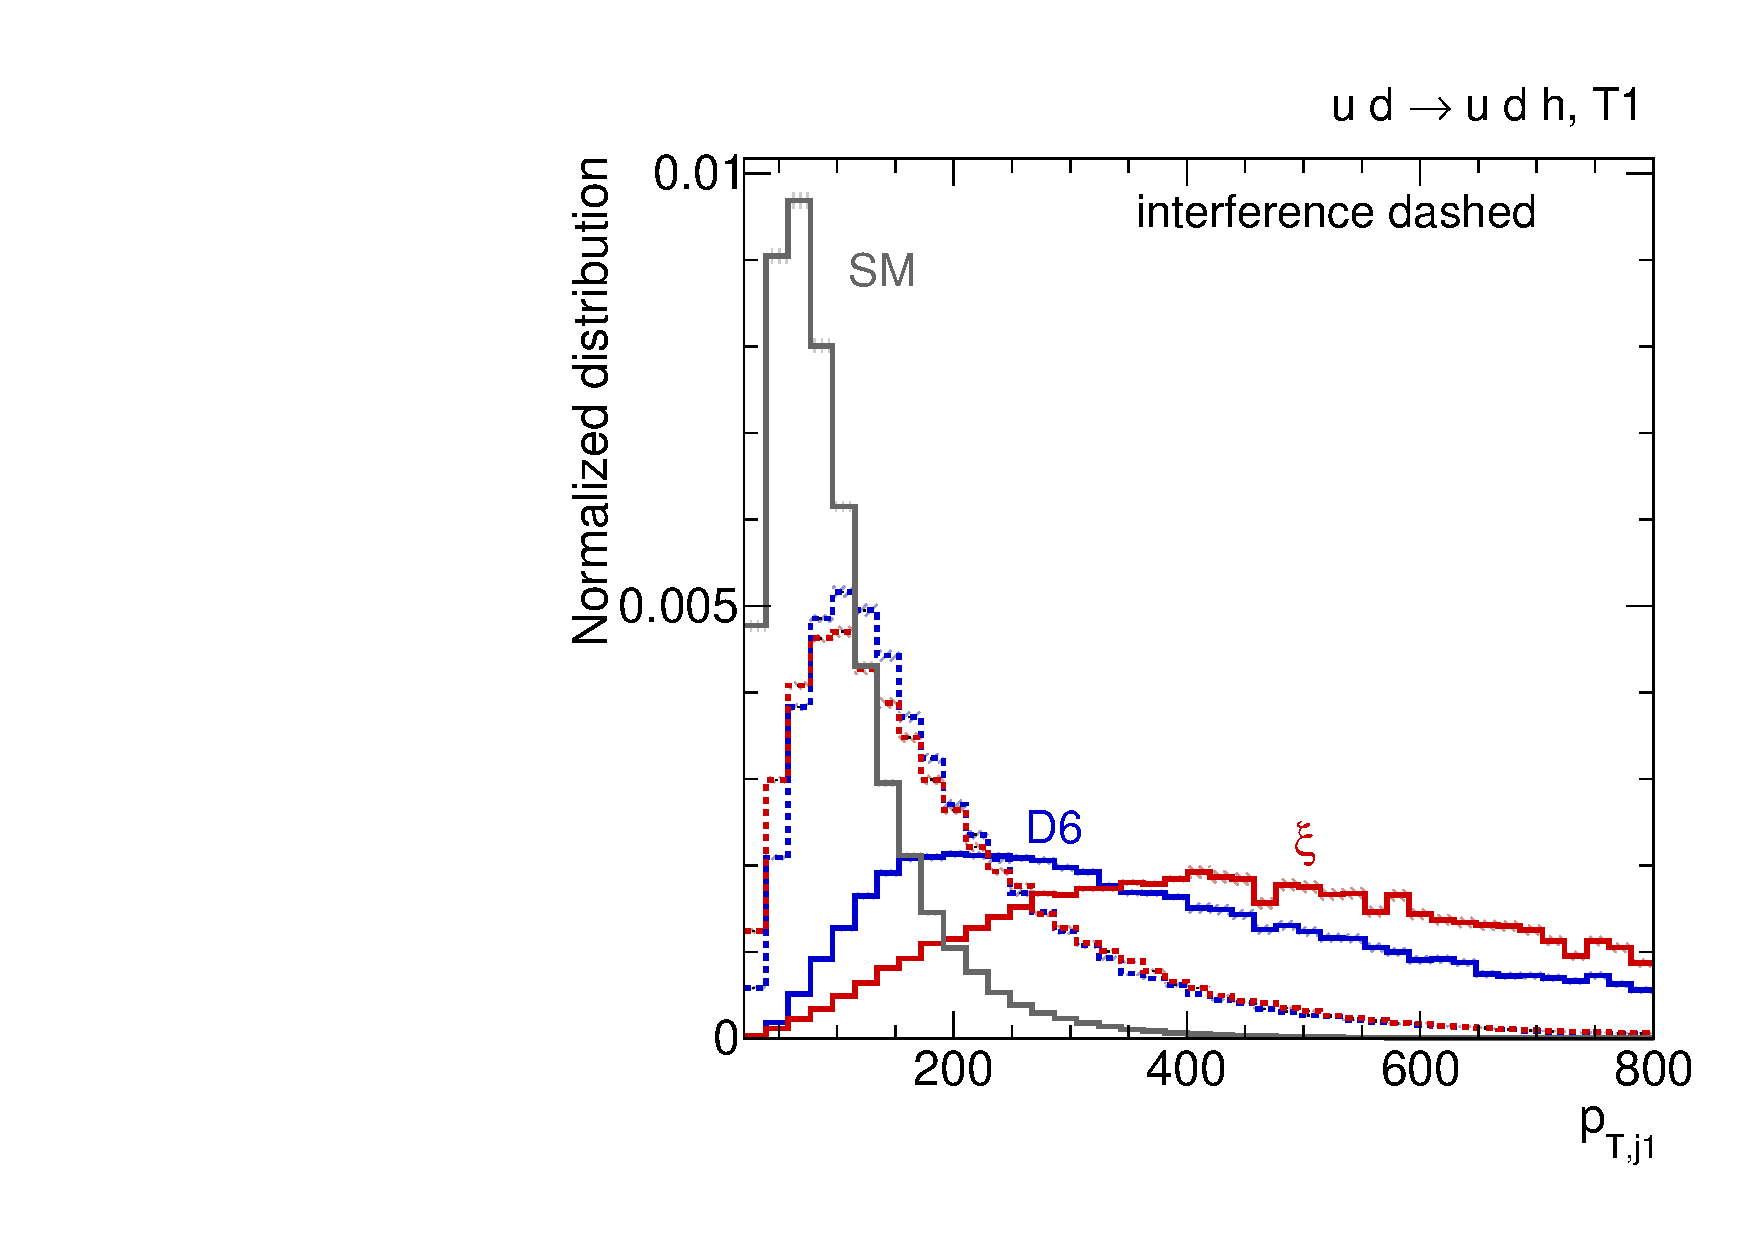
\includegraphics[width=0.49\textwidth]{fig/validity/WBF_separate_T1_j1pt.pdf}%
%   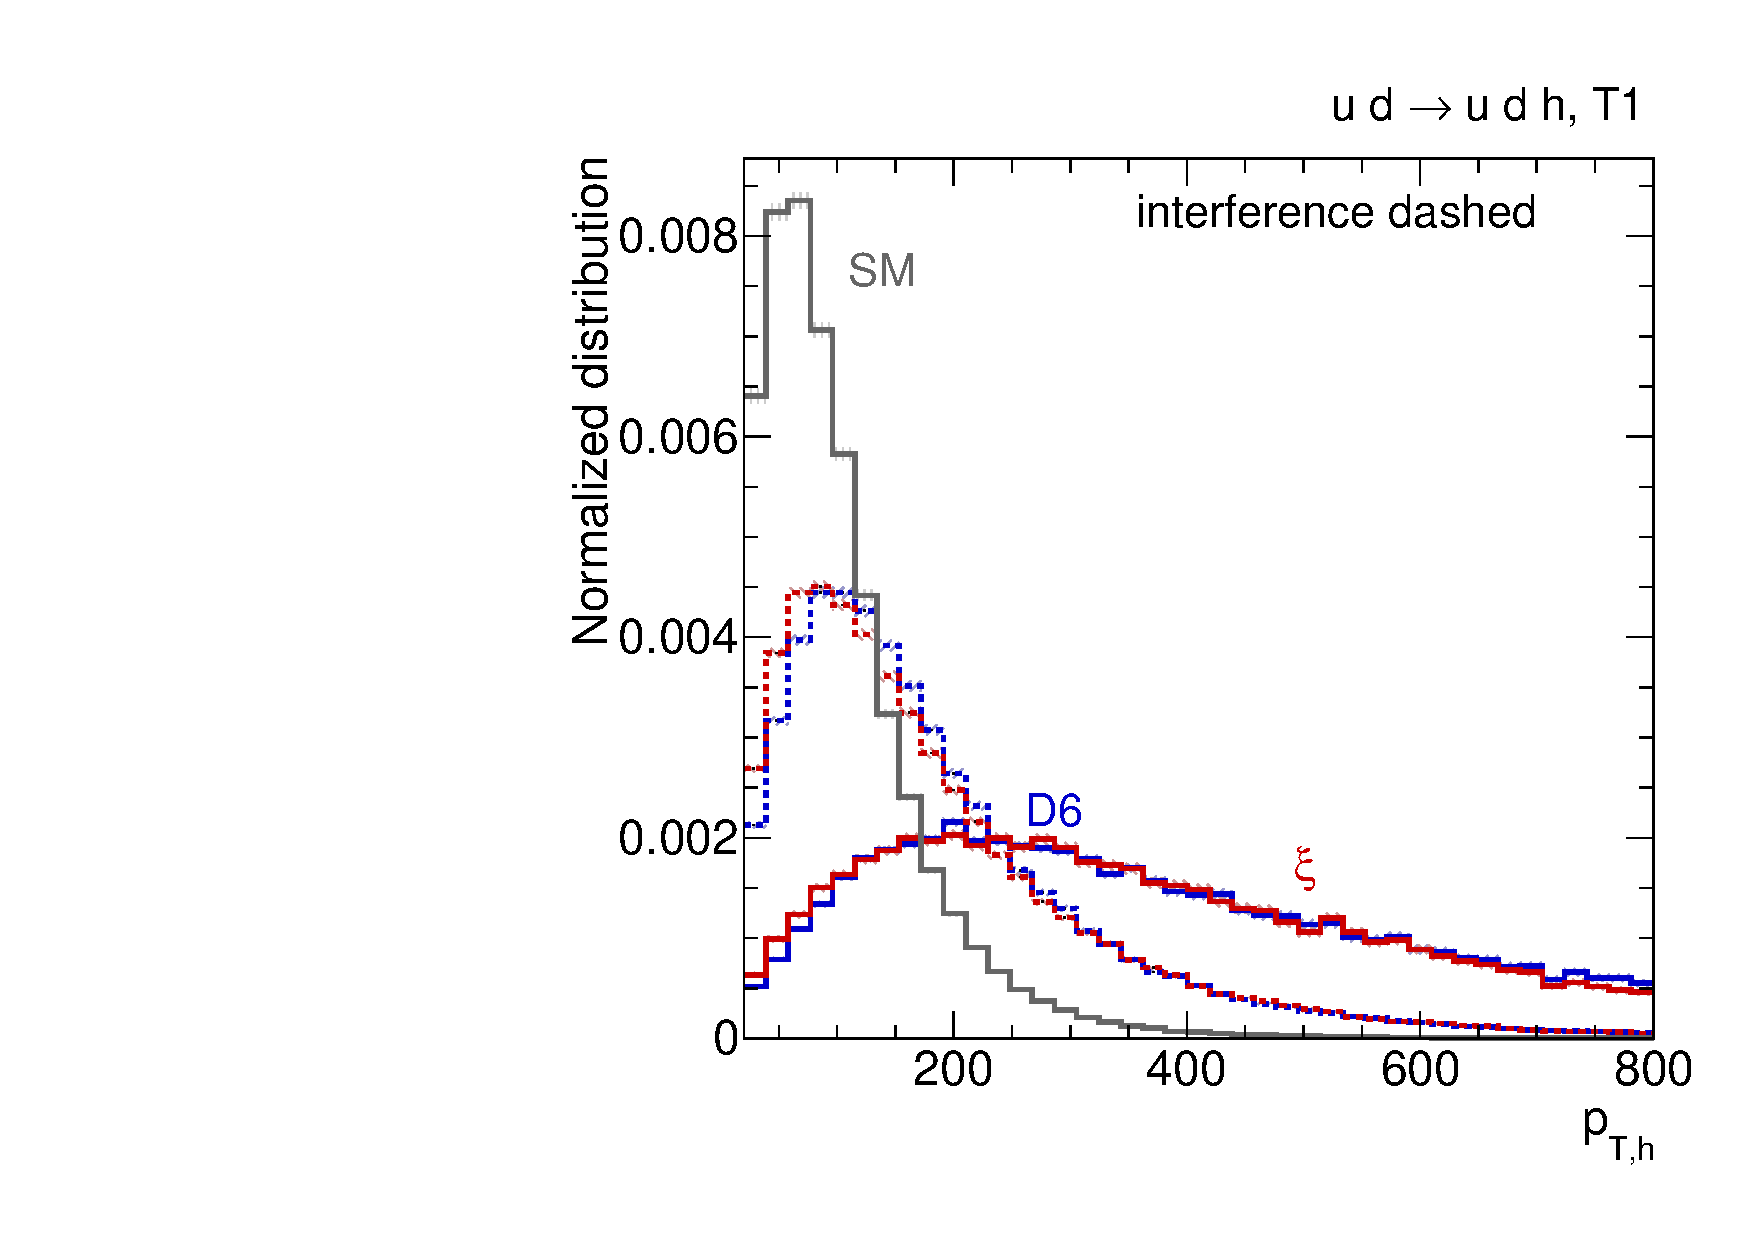
\includegraphics[width=0.49\textwidth]{fig/validity/WBF_separate_T1_Hpt.pdf}\\%
%   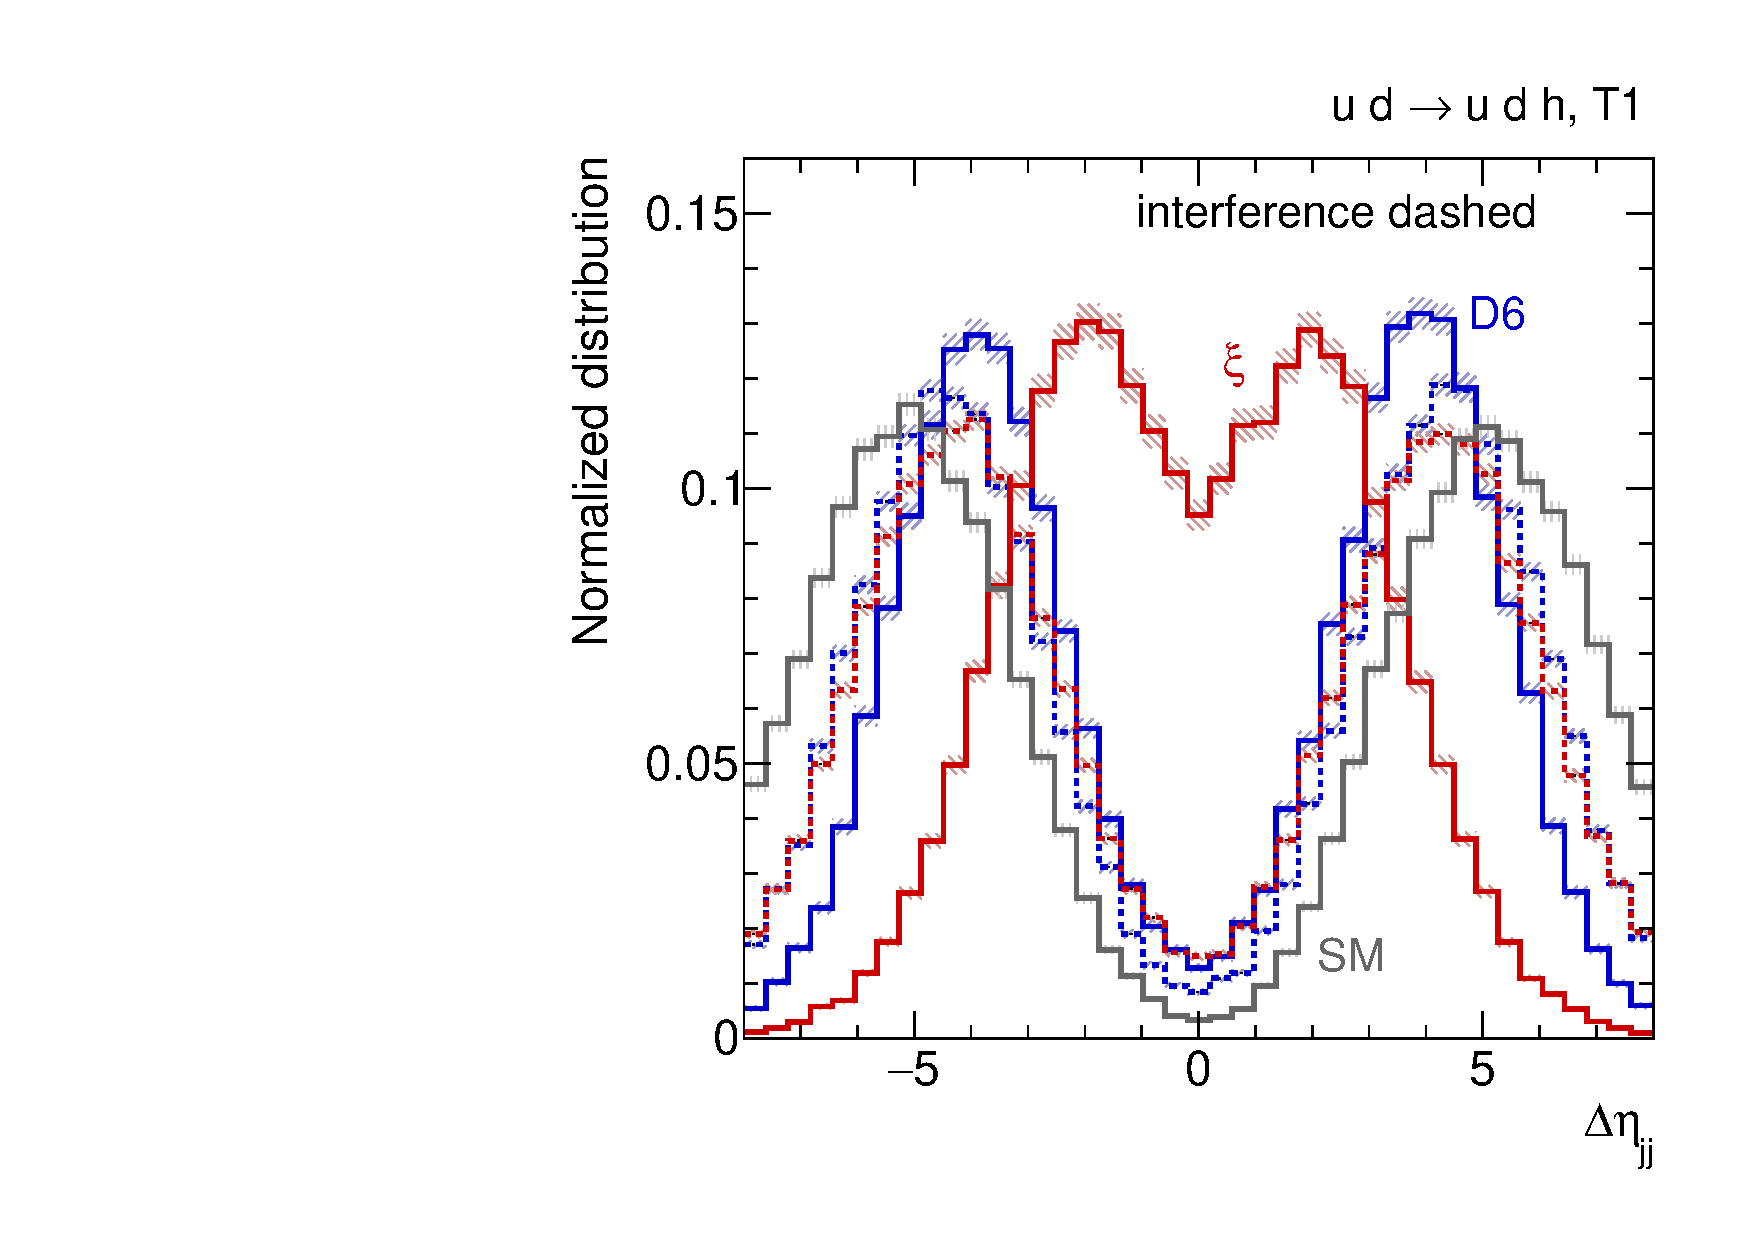
\includegraphics[width=0.49\textwidth]{fig/validity/WBF_separate_T1_deltaEtaJJ.pdf}%
%   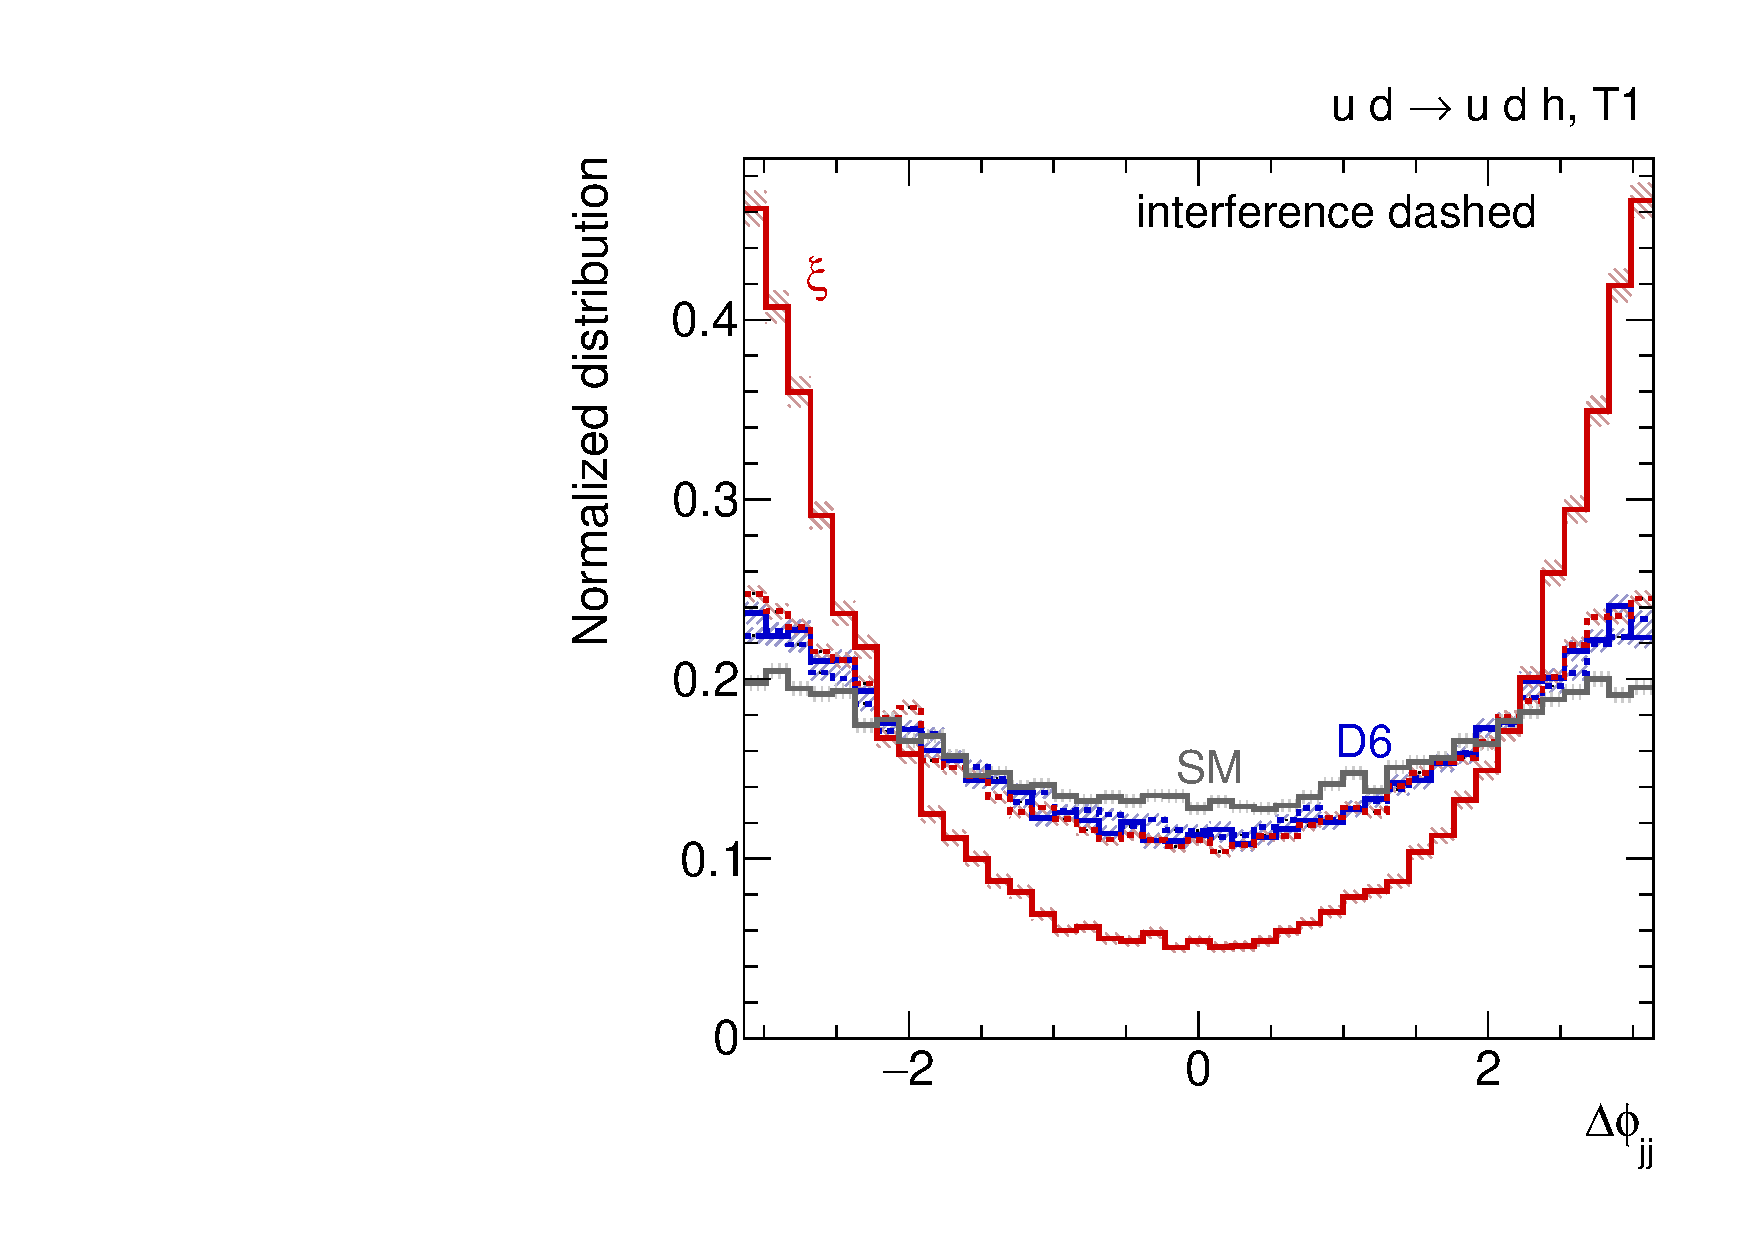
\includegraphics[width=0.49\textwidth]{fig/validity/WBF_separate_T1_deltaPhiJJ.pdf}%
%   \caption{Normalised WBF distributions of the tagging jets. We separate
%     the squared new-physics amplitudes, shown as solid lines, from the
%     interference with the SM-like diagrams (dashed).}
%   \label{fig:validity_squared_separate}
% \end{figure}

% In the first part of the paper we have shown where in phase space a
% dimension-six description of LHC observables breaks down, both for $Vh$
% production and for weak boson fusion. For $Vh$ production with its
% simple $2 \to 2$ kinematics problems are clearly linked to a possible
% $s$-channel resonance, as seen in Equation\;\eqref{eq:validity_breakdown_vh}.  For
% weak boson fusion there appears no resonance, but the result of
% Equation\;\eqref{eq:validity_breakdown_wbf} suggests that the new states in the
% $t$-channel have a similar effect.  In \autoref{fig:validity_squared_separate}
% we show different tagging jet distributions, separating the Feynman
% diagrams including the heavy $\xi$ states. In particular for the
% critical $p_{T,j_1}$ distribution, the $\Delta \eta_{jj}$
% distribution, and the $\Delta \phi_{jj}$ distribution these diagrams
% are only very poorly described by the dimension-six approach. In
% practice this is not a problem because these contributions are
% strongly suppressed by the heavy mass $m_\xi$, but it poses the
% question how we can improve the agreement. The obvious solution to
% these problems in the $s$-channel of $Vh$ production and in the
% $t$-channel of weak boson fusion is a simplified
% model~\cite{simp,simp_higgs}. A new vector field mixing with the weak
% bosons as described by the Lagrangian shown in
% Equation\;\eqref{eq:validity_lag-vectortriplet} is such a simplified model, but its
% structure is still relatively complex. Obviously, an additional heavy
% scalar with mass around $m_\xi$ and the appropriate couplings will
% improve the $2 \to 2$ kinematics for $Vh$ production. The question we
% want to study in this section is if such a scalar can also improve the
% weak boson fusion kinematics.



% %%%%%%%%%%%%%%%%%%%%%%%%%%%%%%%%%%%%%%%%%%%%%%%%%%%%%%%%%%%%
% \subsubsection*{A pseudo-scalar as a simplified vector}
% %%%%%%%%%%%%%%%%%%%%%%%%%%%%%%%%%%%%%%%%%%%%%%%%%%%%%%%%%%%%

% The simplest simplified model we can write down includes one new
% massive scalar $S$ with a Higgs portal and a Yukawa coupling. 
% However, a scalar state will not interfere with the Standard Model
% diagrams. In analogy to the CP properties of the Goldstone mode
% contributing to the massive $Z$ boson we define our simplified model
% with a pseudo-scalar state as
% %
% \begin{align}
% \mathcal{L} \supset 
%   \frac{1}{2} (\partial_\mu S)^2 
% - \frac{m_S}{2} S^2 
% + \sum_\text{fermions} g_F \; S \overline{F} \gamma_5 F 
% + g_S \; S^2 \phi^\dagger \phi \,.
%   \label{eq:validity_simplified_model}
% \end{align}

% %------------------------------------------------------------
% \begin{figure}[t]
%   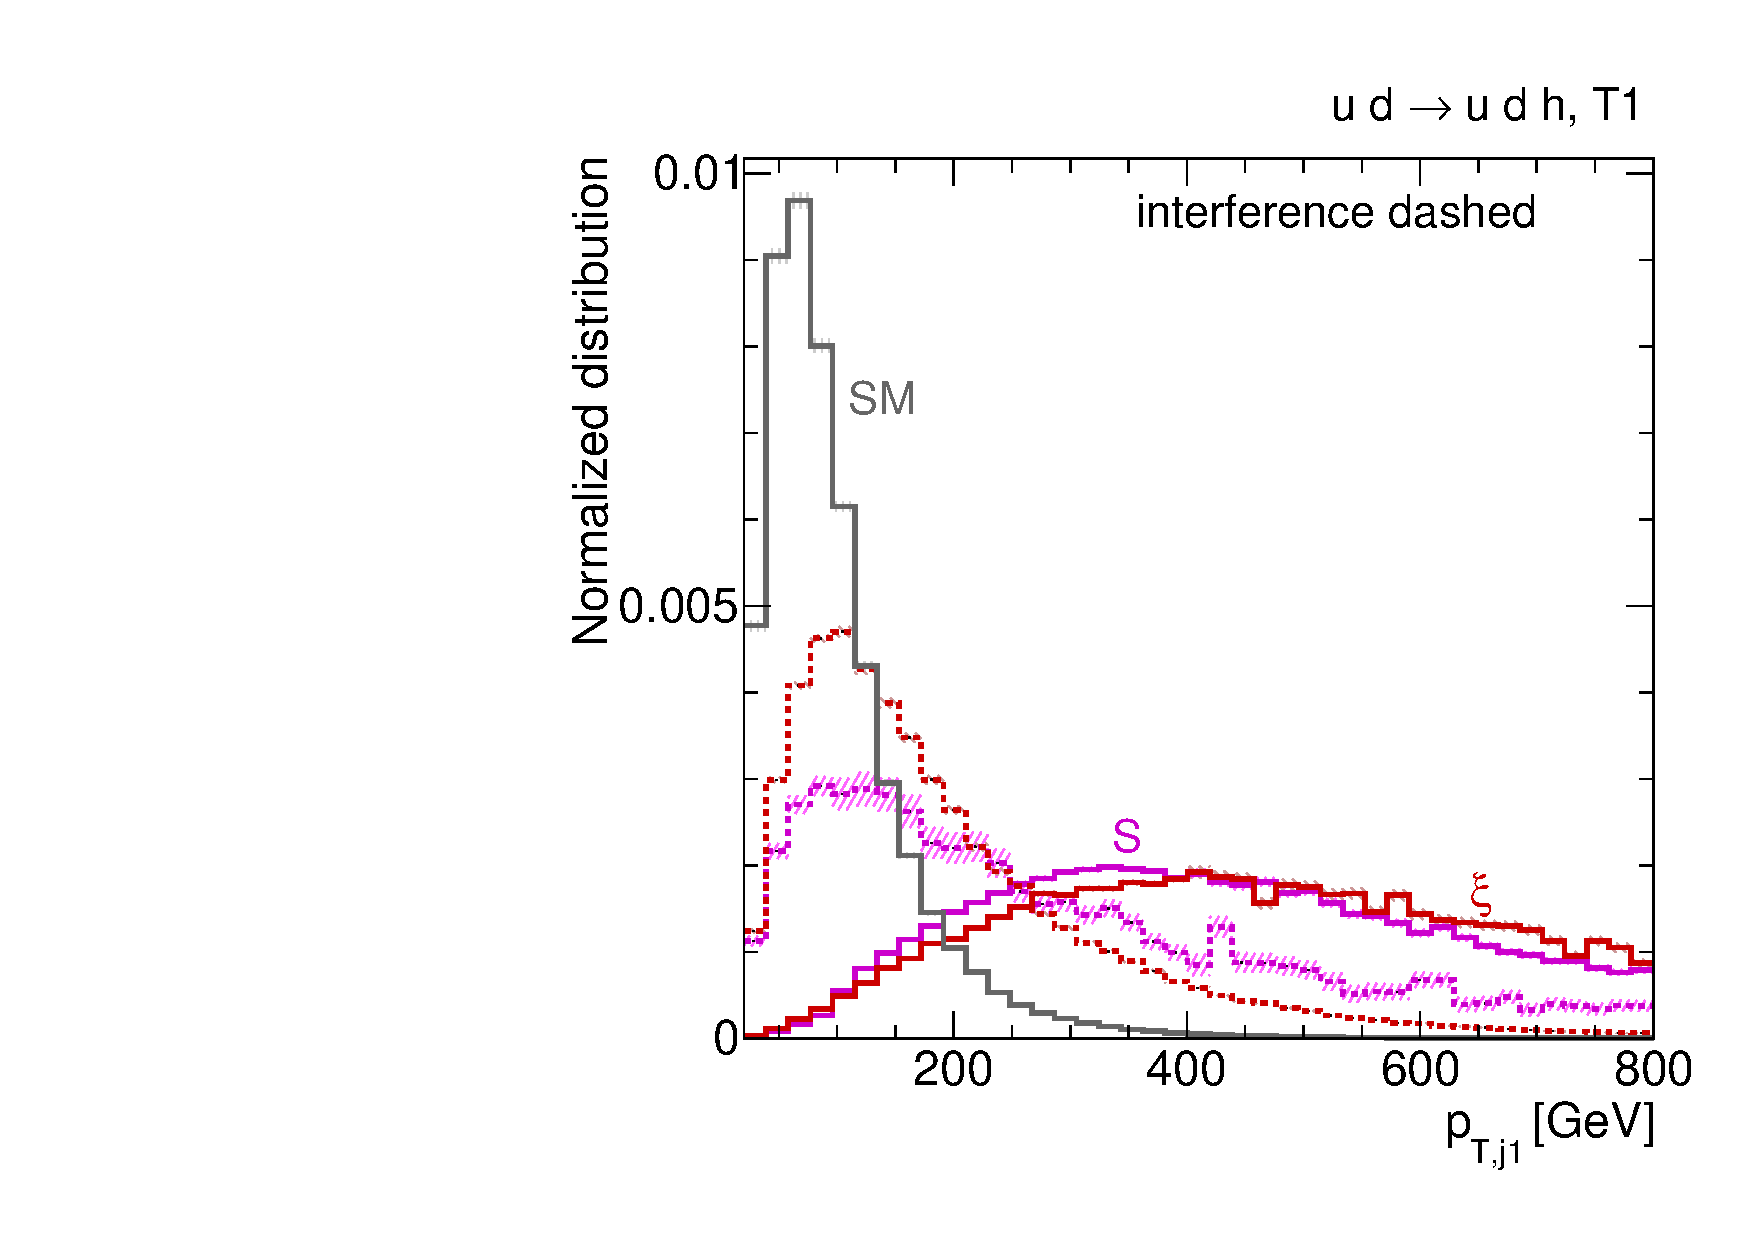
\includegraphics[width=0.43\textwidth]{fig/validity/WBF_simplified_j1pt.pdf}
%   \hspace*{0.05\textwidth}
%   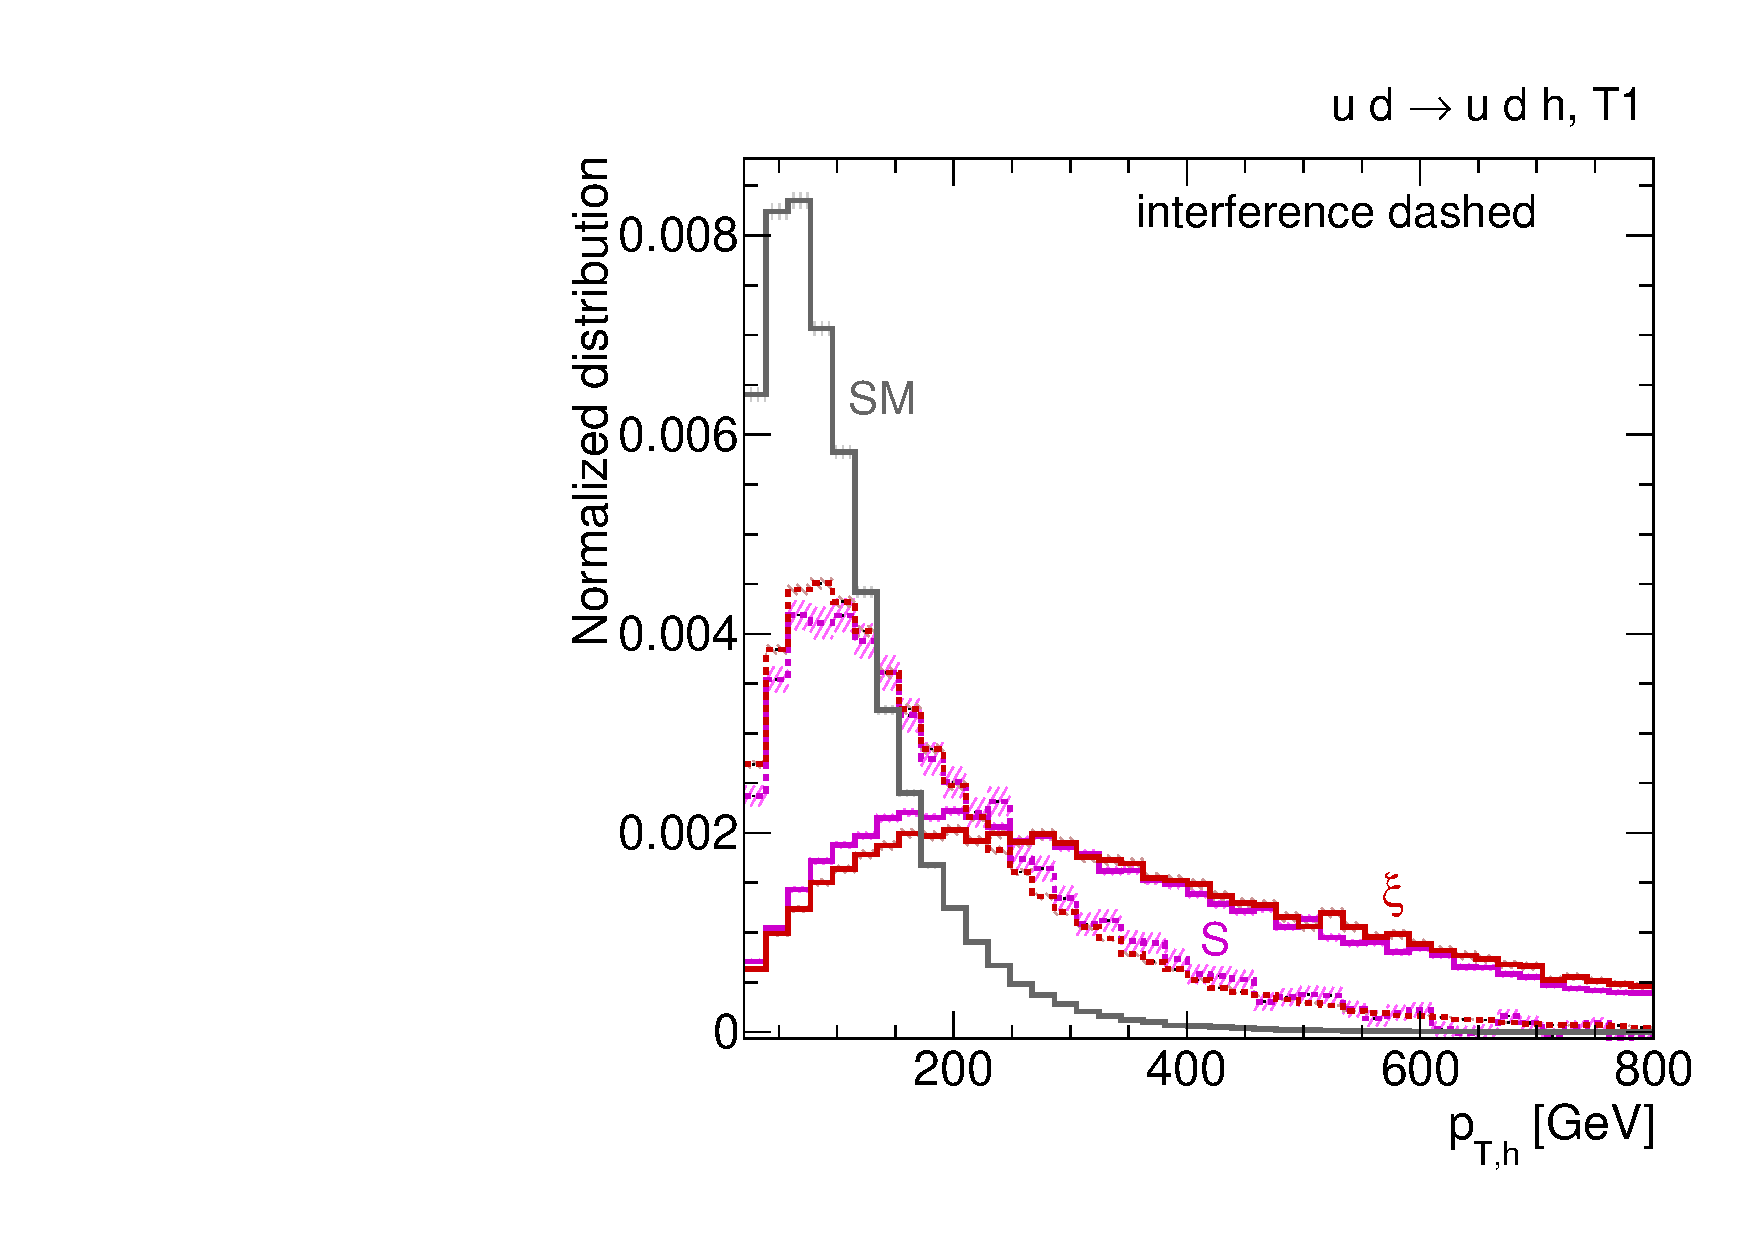
\includegraphics[width=0.43\textwidth]{fig/validity/WBF_simplified_Hpt.pdf} \\
%   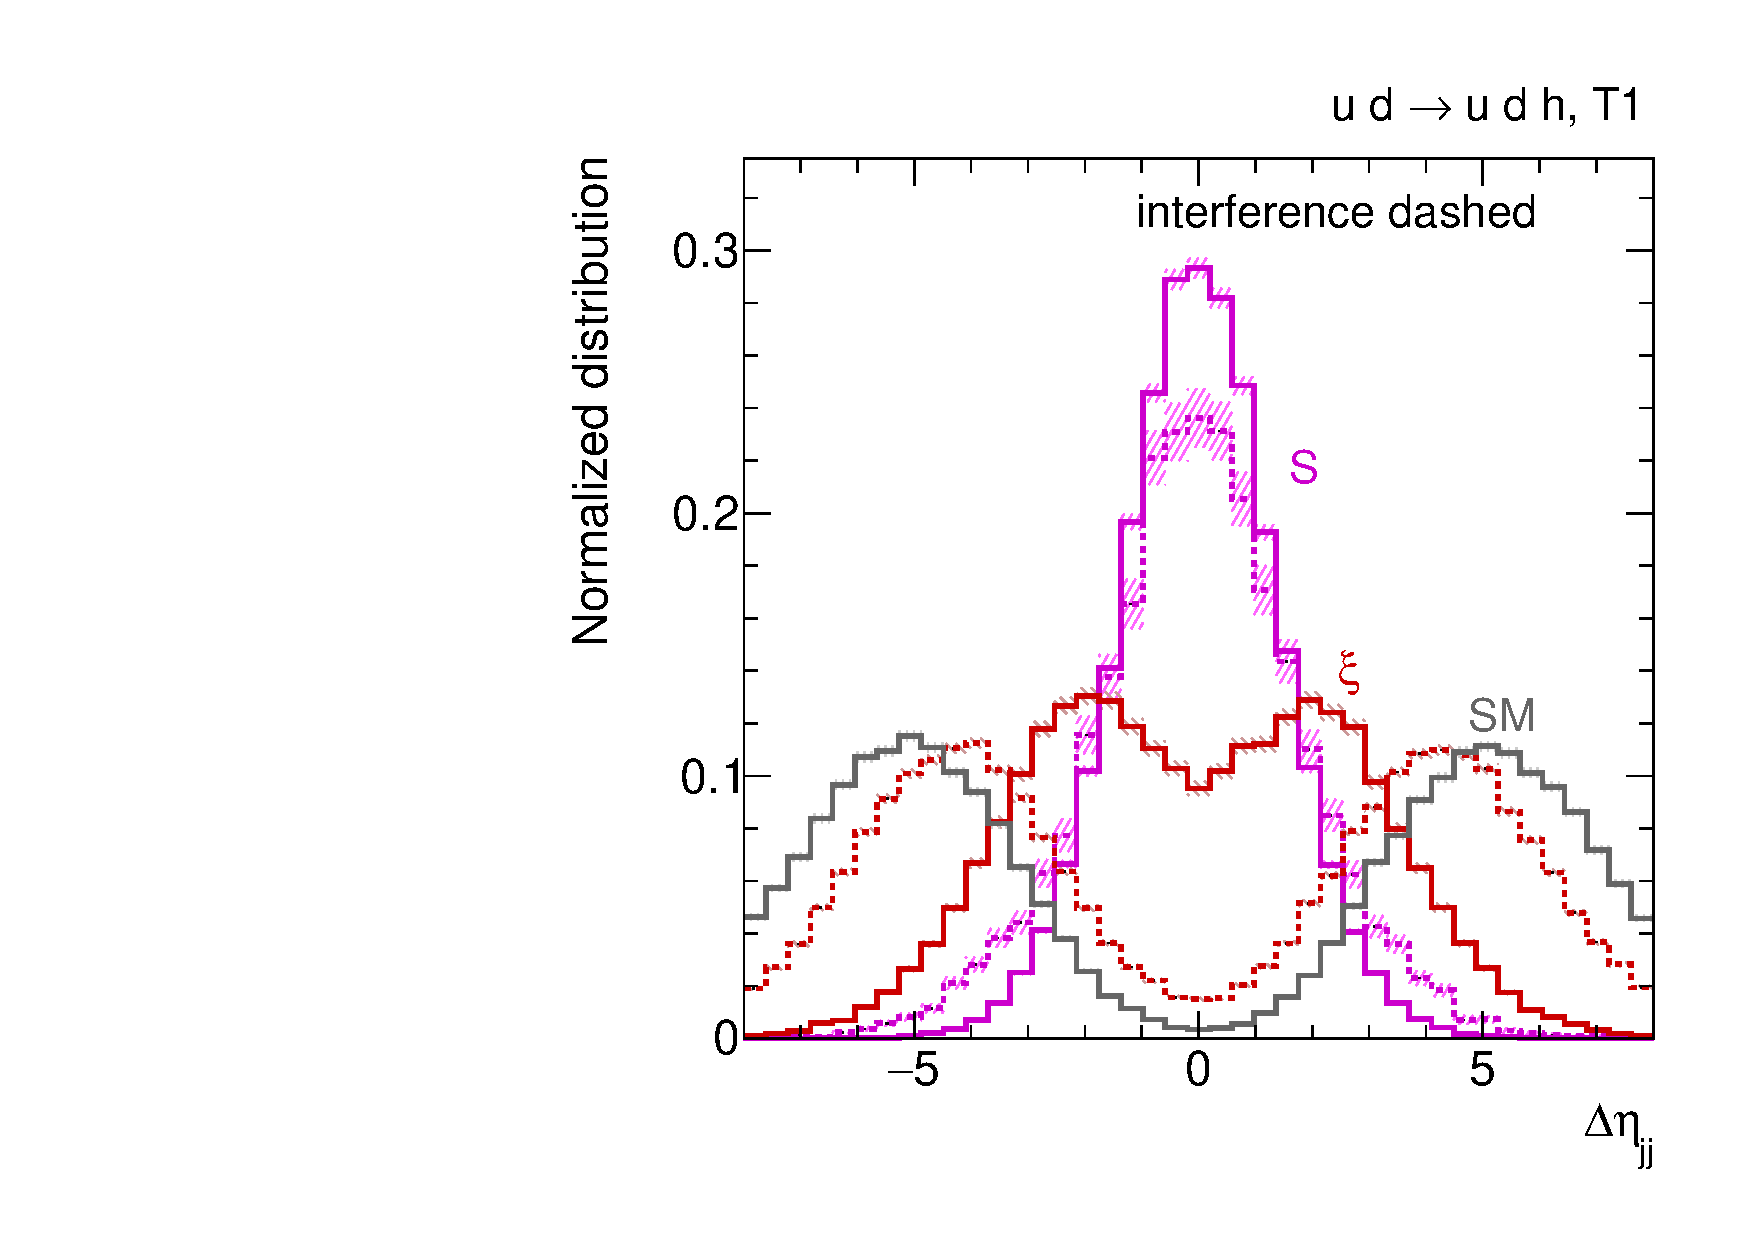
\includegraphics[width=0.43\textwidth]{fig/validity/WBF_simplified_deltaEtaJJ.pdf}
%   \hspace*{0.05\textwidth}
%   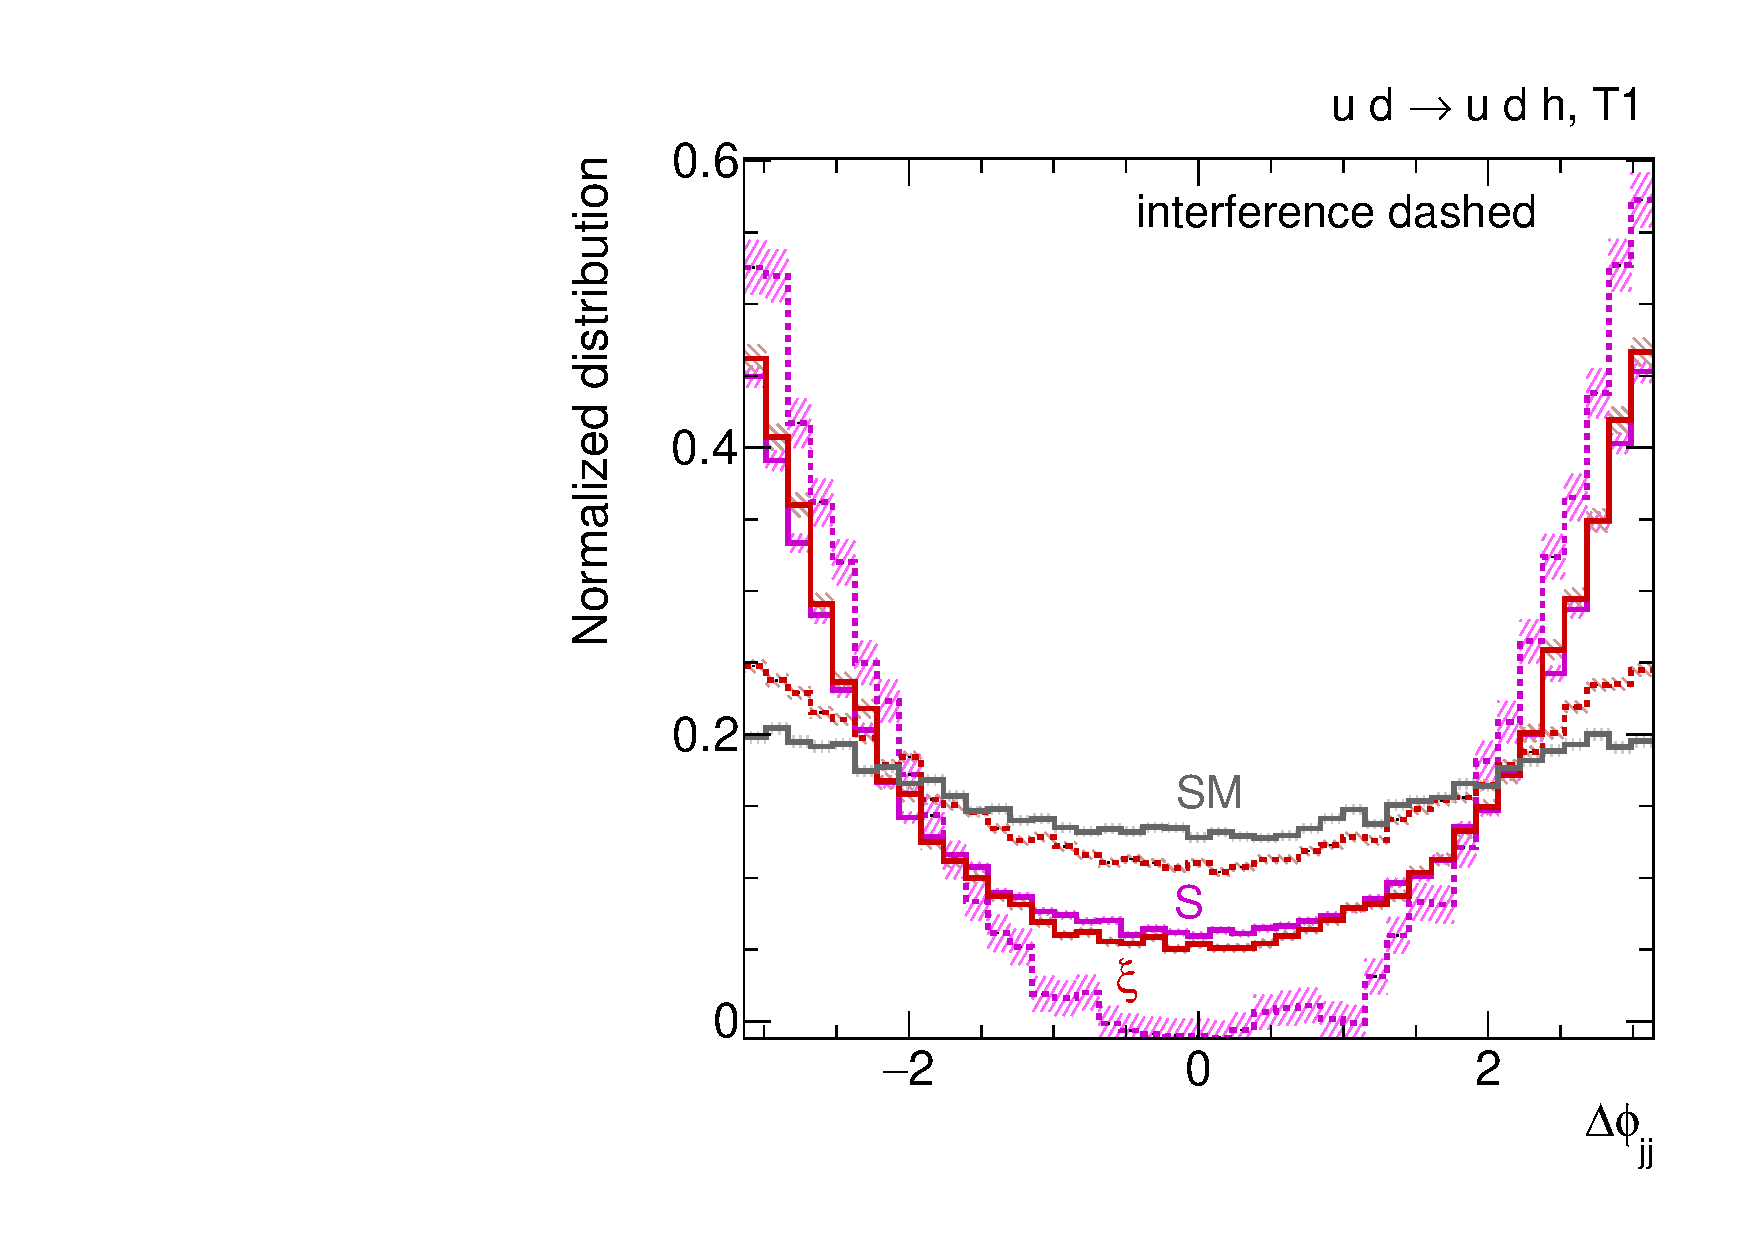
\includegraphics[width=0.43\textwidth]{fig/validity/WBF_simplified_deltaPhiJJ.pdf}
%   \caption{Normalised WBF distributions for a scalar simplified model
%     defined in Equation\;\eqref{eq:validity_simplified_model} vs the vector triplet
%     benchmark.}
%   \label{fig:validity_simplified}
% \end{figure}
% %------------------------------------------------------------

% In \autoref{fig:validity_simplified} we show the same WBF distributions as in
% \autoref{fig:validity_squared_separate}, but including the simplified scalar
% model. For the $p_{T,j}$ distribution the squared new-physics
% amplitudes in the full vector model and the simplified scalar model
% indeed agree well, improving upon the dimension-six description which
% breaks down in this distribution.  However, the interference term with
% the Standard Model, which is numerically dominant for most of the
% distribution and well described in the dimension-six model, poses a
% problem.  The $\Delta \eta_{jj}$ distributions show even poorer
% agreement: the spin-1 amplitudes of the Standard Model and the vector
% triplet have similar phase-space distributions and give two forward
% tagging jets, while the scalar mediator favours central
% jets~\cite{spins2}.  The $\Delta \phi_{jj}$ distribution, known to be
% sensitive to the tensor structure of the hard $VVh$
% interaction~\cite{delta_phi}, exposes similar differences between the
% full and simplified model.  Altogether, our simplified scalar model
% with its very different $VVh$ interaction structure does improve the
% description in the region where the dimension-six approach breaks down,
% but it fails to describe interference patterns and angular
% correlations of the tagging jets.



% %%%%%%%%%%%%%%%%%%%%%%%%%%%%%%%%%%%%%%%%%%%%%%%%%%%%%%%%%%%%
% \subsubsection*{Splitting functions and equivalence theorem}
% %%%%%%%%%%%%%%%%%%%%%%%%%%%%%%%%%%%%%%%%%%%%%%%%%%%%%%%%%%%%

% We can understand this very different behaviour of the scalar
% $t$-channel mediator as compared to the vector from the splitting
% kernels in the collinear limit.  The matrix element squared for the
% weak boson fusion process mediated by pseudo-scalars $S$ has the form
% %
% \begin{align}
%  | \mathcal{M}(qq \to q'q'h) |^2 \propto 
%   \frac{g_F^4 \;  t_1 t_2}{(t_1 - m_S^2)^2 \; (t_2 - m_S^2)^2} 
% \stackrel{m_S \to 0}{\longrightarrow} \frac{\text{const}}{t_1 t_2} \; ,
% \end{align}
% %
% where $t_1$ and $t_2$ denote the respective momentum flow through each
% scalar propagator. For $m_S \to 0$ the Jacobians from the phase-space
% integration cancel a possible collinear divergence, while for a light
% vector boson a soft and a collinear divergence remains. Unlike in the
% usual WBF process, the tagging jets in our simplified scalar model
% will not be forward.  The reason for this difference in the
% infrared is the (pseudo-)scalar coupling to quarks: since the scalar
% carries no Lorentz index, a $q \to q S$ splitting will be expressed in
% terms of the momentum combinations $(p_q p_q')$, $p_q^2 = m_q^2$, and
% $p_q'^2 = m_q^2$. In the limit of massless quarks only the first term
% remains as $t = 2 (p_q p_q')$.  This factor in the numerator cancels
% the apparent divergence of the $t$-channel propagator.

% Adding higher-dimensional couplings of the (pseudo-)scalar to
% fermions, such as
% %
% \begin{align}
%   \mathcal{L} \supset 
% \sum_\text{fermions} \Biggl[  
%   g_{F,2} S \overline{F} F 
% + g_{F,3} (\partial_\mu S) \overline{F} \gamma^\mu F
% + g_{F,4} S (\partial_\mu S) \overline{F} \gamma^\mu \gamma_5 F 
% + g_{F,5} S (\partial_\mu \partial_\nu S) \overline{F} [\gamma^\mu,\gamma^\nu] F
% \Biggr] \; ,
% \label{eq:validity_simplified_model_extended}
% \end{align}
% %
% does not change this result qualitatively. After partial integration
% and using the Dirac equation for the on-shell quarks the coupling
% $g_{F,3}$ is equivalent to the simple scalar coupling, $g_{F,2} = m_q^2
% g_{F,3}$. In the limit of massless quarks, only two of the new
% structures listed in Equation\;\eqref{eq:validity_simplified_model_extended}
% contribute at all: $g_{F,2}$ gives exactly the same result as $g_F$,
% while $g_{F,5}$ leads to even higher powers of $t$ in the numerator,
% %
% \begin{align}
%   | \mathcal{M}(qq \to q'q'h) |^2 \propto 
%   \frac{g_{F,5}^4 \; t_1^3 t_2^3}{(t_1 - m_s^2)^2 \; (t_2 - m_s^2)^2} \; . 
% \end{align}
% %
% No matter how we couple the (pseudo-)scalar of the simplified model to
% the external quarks, it never reproduces the collinear splitting
% kernel of a vector boson.

% To be a little more precise, we can write out the spin-averaged matrix
% element squared for the $q \to q' S$ splitting in terms of the energy
% of the initial quark $E$, the longitudinal momentum fraction $x$, and
% the transverse momentum $p_T$, both carried by $S$,
% %
% \begin{align}
%  | \mathcal{M}(q \to q'S) |^2 &= - 2 g_F^2 x m_q^2
%                      + 2 g_F^2 E^2 (1-x)
%                      \Biggl[ \sqrt{1 + \frac {p_T^2} {E^2 (1-x)^2} + \frac {m_q^2 (1 - (1-x)^2)} {E^2 (1-x)^2} } - 1 \Biggr] \notag \\
%                    &= g_F^2 \, \frac {x^2 \, m_q^2} {1-x} 
%                      + g_F^2 \,  \frac {p_T^2} {1-x} 
%                      + \ord { \frac{m_q^2 p_T^2}{E^2}, \frac{m_q^4}{E^2}, \frac{p_T^4}{E^2} } \;.
% \label{eq:validity_splitting_s}
% \end{align}
% %
% From Equation\;\eqref{eq:validity_splitting_s} one can derive an effective Higgs
% approximation or \emph{effective scalar
%   approximation}~\cite{effective_scalar}: in the collinear and
% high-energy limit, a process $q X \to q' Y$ mediated by a
% (pseudo-)scalar $S$ is described by
% %
% \begin{align}
%   \sigma (qX \to q'Y) = \int \mathrm{d}x \, \mathrm{d} p_T \, F_S(x,p_T)
%   \, \sigma (SX \to Y)
% \label{eq:validity_def_splitting}
% \end{align}
% %
% with the splitting function
% %
% \begin{align}
%   F_S(x,p_T) &= \frac {g_F^2} {16 \pi^2} \, 
%                \frac {x \, p_T^3} {\left( m_S^2 (1-x) + p_T^2 \right)^2} \,.
% \label{eq:validity_kernel_s}
% \end{align}
% %
% Unlike for vector emission, there is no soft divergence for $x \to 0$.
% The $p_T$ dependence is the same as for transverse vector
% bosons~\cite{effective_w,polarized_ww}, as we discuss in some detail in the
% appendix. 

% It might seem surprising that our pseudo-scalar is emitted with a
% fundamentally different phase-space dependence than longitudinal $W$
% and $Z$ bosons, in apparent contradiction of the Goldstone boson
% equivalence theorem.  However, the latter only makes a statement about
% the leading term in an expansion in $m_W / E$, where 
% $\varepsilon^\mu_L \sim p^\mu / m_W$. At this order the squared matrix
% element for the splitting $q \to q' W_L$ agrees with the pseudo-scalar
% result, but is suppressed by a factor of $m_q^2 / E^2$. Higher orders
% in the $m_W/E$ expansion, outside the validity range of the
% equivalence theorem, are not suppressed by quark masses.  The
% equivalence theorem is therefore of very limited use in describing the
% $W$ or $Z$ couplings to quarks except the top.

% %%%%%%%%%%%%%%%%%%%%%%%%%%%%%%%%%%%%%%%%

% In Sec.~\ref{sec:validity_simplified} we have introduced a pseudo-scalar in the
% $t$-channel of weak boson fusion to describe some of the features
% which we find in the full vector triplet model and which our
% dimension-six description does not describe well. In this appendix we
% collect some of the main formulas and compare the kinematics of
% fermions radiating scalars, transverse, or longitudinal gauge
% bosons. Our formalism follows the effective
% $W$ approximation~\cite{effective_w} as well as the effective Higgs
% approximation~\cite{effective_scalar} and allows us to analytically
% describe the soft and collinear behaviour. If we do not need to
% describe interference terms with SM gauge bosons we can start with a
% CP-even scalar splitting $q \to qS$, in terms of the energy of the
% initial quark $E$, the longitudinal momentum fraction $x$, carried by $S$, and the
% scalar's transverse momentum $p_T$:
% %
% \begin{align}
%  | \mathcal{M}(q \to q'S)  |^2 &= 2 g_F^2 (2-x) m_q^2
%                      + 2 g_F^2 E^2 (1-x)
%                      \Biggl[ \sqrt{1 + \frac {p_T^2} {E^2 (1-x)^2} + \frac {m_q^2 (1 - (1-x)^2)} {E^2 (1-x)^2} } 
%                        - 1 \Biggr] \notag \\
%                    &= g_F^2 \left( 4  + \frac {x^2} {1-x} \right) m_q^2
%                      + g_F^2 \, \frac {p_T^2} {1-x} 
%                      + \ord {\frac{m_q^2 p_T^2}{E^2}, \frac{m_q^4}{E^2}, \frac{p_T^4}{E^2} } \; .
% \end{align}
% %
% The main feature of this splitting is that the infrared behaviour is
% different for the term proportional to the quark mass and for the
% surviving term in the realistic limit $m_q \to 0$: in the absence of a
% fermion mass the collinear divergence from a $t$-channel propagator is
% cancelled by the coupling structure. If the term proportional to $m_q$
% dominates there will be the usual collinear divergence once we include
% a scalar propagator. For a pseudo-scalar the structure shown in
% Equation\;\eqref{eq:validity_splitting_s} is very similar,
% %
% \begin{align}
%  |\mathcal{M}(q \to q'S)  |^2 &= - 2 g_F^2 x m_q^2
%                      + 2 g_F^2 E^2 (1-x)
%                      \Biggl[ \sqrt{1 + \frac {p_T^2} {E^2 (1-x)^2} + \frac {m_q^2 (1 - (1-x)^2)} {E^2 (1-x)^2} } 
%                                 - 1 \Biggr] \notag \\
%                    &= g_F^2 \, \frac {x^2 \, m_q^2} {1-x} 
%                      + g_F^2 \,  \frac {p_T^2} {1-x} 
%                      + \ord {\frac{m_q^2 p_T^2}{E^2}, \frac{m_q^4}{E^2}, \frac{p_T^4}{E^2} } \;.
% \end{align}

% In the limit $m_q \to 0$ we can compute universal splitting kernels
% including only the leading term in $p_T$, as defined in
% Equation\;\eqref{eq:validity_def_splitting}.  Obviously, the scalar and pseudoscalar
% case given in Equation\;\eqref{eq:validity_kernel_s} are identical, and we can compare
% them with the splitting kernels for longitudinal or transverse
% $W$ bosons~\cite{effective_w},
% %
% \begin{align}
%   F_S(x,p_T) &= \frac {g_F^2} {16 \pi^2} \, x \,
%                \frac {p_T^3} {\left( m_S^2 (1-x) + p_T^2 \right)^2} \,,\notag \\
%   F_T(x,p_T) &= \frac {g^2} {16 \pi^2} \, \frac {1+(1-x)^2} x \, \frac {p_T^3} {\left( m_W^2 (1-x) + p_T^2 \right)^2} \,, \notag \\
%   F_L(x,p_T) &= \frac {g^2} {16 \pi^2} \, \frac {(1-x)^2} x \, \frac {2 m_W^2 \, p_T} {\left( m_W^2 (1-x) + p_T^2 \right)^2} \,.
%   \label{eq:validity_splittings}
% \end{align}

% In \autoref{fig:validity_effective_scalar} we show how these different
% splittings translate into WBF distributions and compare full simulations
% in \toolfont{MadGraph} to the predictions of Equation\;\eqref{eq:validity_splittings}.
% A heavy Higgs, $m_h = 1$~TeV, is needed to guarantee a large energy scale
% $E \sim m_h \gg p_T \sim m_W, m_S$. In this case we find that the
% effective scalar approximation quite accurately describes the transverse
% momentum distribution of the tagging jets. For $m_h = 125$~GeV the
% assumption of on-shell $W$ bosons or scalars breaks down and the
% effective descriptions lose their validity.

% \begin{figure}
%   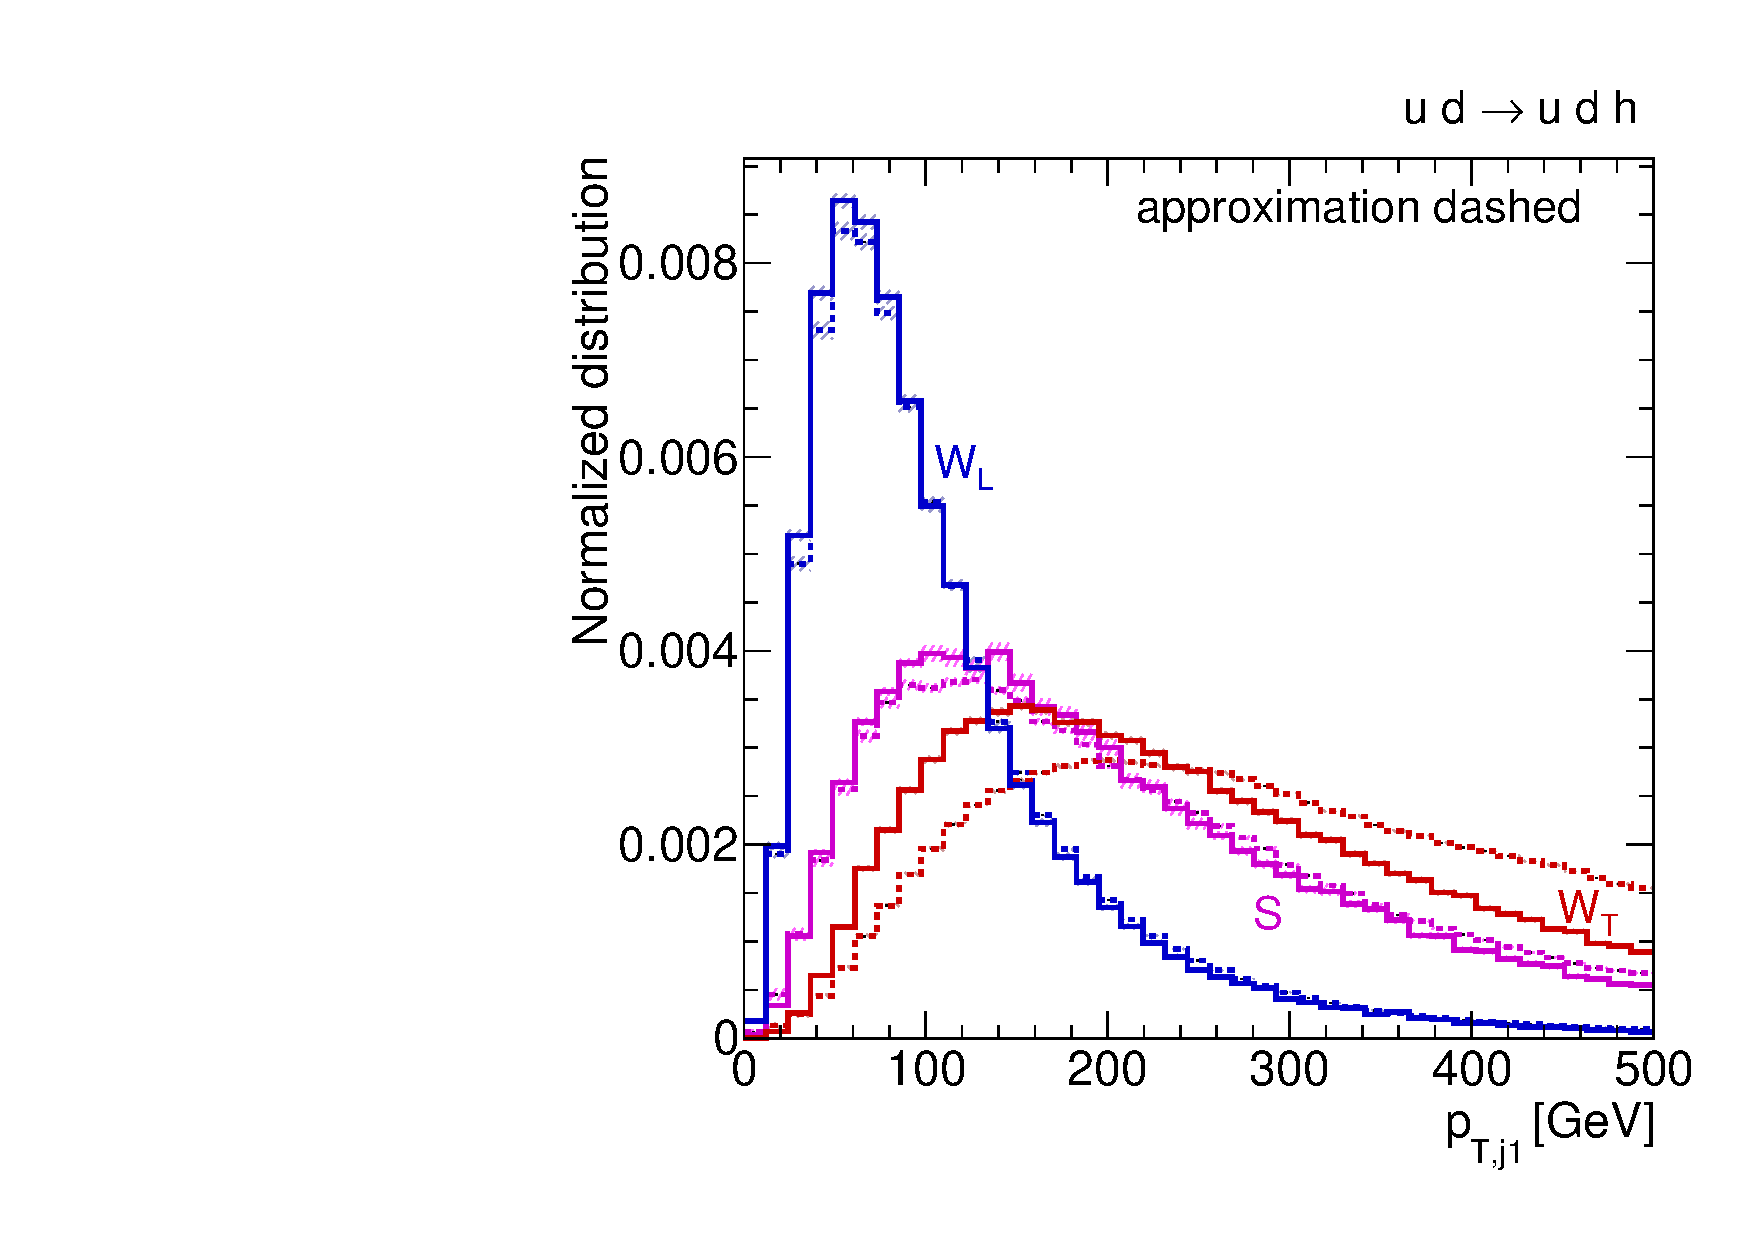
\includegraphics[width=0.43\textwidth]{fig/validity/WBF_ESA.pdf}
%   \caption{Normalised WBF distributions of the tagging jets in the SM with
%   a heavy Higgs, $m_h = 1$~TeV. Scalar mediators are compared to
%   longitudinal and transverse $W$ bosons following
%   Reference~\cite{polarized_ww}.
%   The dotted lines give the corresponding predictions of the effective
%   $W$ and scalar approximations, \autoref{eq:validity_splittings}.}
%   \label{fig:validity_effective_scalar}
% \end{figure}





%%%%%%%%%%%%%%%%%%%%%%%%%%%%%%%%%%%%%%%%%%%%%%%%%%%%%%%%%%%%
\section{Information geometry}
\label{sec:appendix_information}
%%%%%%%%%%%%%%%%%%%%%%%%%%%%%%%%%%%%%%%%%%%%%%%%%%%%%%%%%%%%



%%%%%%%%%%%%%%%%%%%%%%%%%%%%%%%%%%%%%%%%%%%%%%%%%%%%%%%%%%%%
\subsection{Cram\'er-Rao bound}
\label{sec:appendix_information_cramer_rao}
%%%%%%%%%%%%%%%%%%%%%%%%%%%%%%%%%%%%%%%%%%%%%%%%%%%%%%%%%%%%

In \autoref{eq:information_cramer_rao_general} in
\autoref{sec:information_formalism} we stated the Cram\'er-Rao
bound~\cite{Rao:1945, Cramer:1946}: the covariance of any estimator is
bounded from below by the inverse Fisher information. Here we show the
proof for the one-dimensional case and unbiased estimators, closely
following Reference~\cite{Watkins:statistics}.

An unbiased estimator $\hat{\theta}(\boldx)$ based on data $\boldx$
has an expectation value equal to the unknown true value $\theta$,
%
\begin{equation}
  \theta = E \left [ \hat{\theta} \middle | \theta \right]
  \equiv \intfatx \hat{\theta} \; f(\boldx|\theta) \,.
  \label{eq:appendix_information_cramer_rao_proof_unbiased}
\end{equation}
%
Like any probability distribution function, $f(\boldx|\theta)$ is normalised to one,
%
\begin{equation}
  1 = \intfatx f(\boldx|\theta) \,. 
  \label{eq:appendix_information_cramer_rao_proof_norm}
\end{equation}
%
We assume that these two equations are differentiable with respect to
$\theta$, and that we can exchange this derivative with the
integral. Differentiating
\autoref{eq:appendix_information_cramer_rao_proof_norm} with respect
to $\theta$ gives
%
\begin{align}
  0 &= \intfatx \partial_\theta f(\boldx|\theta) \notag \\
  &= \intfatx \frac{\partial_\theta f(\boldx|\theta)} {f(\boldx|\theta)} \; f(\boldx|\theta) \notag \\
  &= E \left[ \partial_\theta \log f(\boldx|\theta) \middle| \theta  \right] \,. 
  \label{eq:appendix_information_cramer_rao_proof_score}
\end{align}
%
For \autoref{eq:appendix_information_cramer_rao_proof_unbiased} we find in the same way
%
\begin{align}
  1 &= \intfatx \hat{\theta} \partial_\theta f(\boldx|\theta) \notag \\
  &= E \left[ \hat{\theta} \; \partial_\theta \log f(\boldx|\theta) \middle| \theta \right] \,. 
  \label{eq:appendix_information_cramer_rao_proof_intermediate1}
\end{align}
%
We can phrase this in terms of the covariance
%
\begin{equation}
  \cov \left[ X,Y \middle| \theta \right]
  \equiv E \left[ (X - E[X|\theta]) (Y - E[Y|\theta]) \middle| \theta \right]
  = E \left[ XY \middle| \theta \right] - E\left[X \middle| \theta \right] \, E\left[Y \middle| \theta \right]
\end{equation}
%
(which is closely related, but not identical, to the covariance matrix
defined in \autoref{eq:information_covariance_matrix}).  Using
\autoref{eq:appendix_information_cramer_rao_proof_score},
\autoref{eq:appendix_information_cramer_rao_proof_intermediate1} can
then be written as
%
\begin{equation}
  1 = \cov \left[ \hat{\theta} , \partial_\theta \log f(\boldx|\theta) \middle| \theta \right] \,. 
  \label{eq:appendix_information_cramer_rao_proof_intermediate2}
\end{equation}
%
We can square this equation and apply the Cauchy-Schwartz
identity\footnote{This inequality is well-known in the form of the
  bounds on the Pearson correlation coefficient, $-1 \leq r \leq 1$
  with $r = \cov [X,Y] / \sqrt{\var[X]\,\var[Y]}$.}
%
\begin{equation}
  \cov [X, Y]^2 \geq \var [X] \, \var[Y] \,,
\end{equation}
%
leading to
%
\begin{equation}
  1 \leq \var \left[ \hat{\theta} \middle| \theta \right] \; \var \left[ \partial_\theta \log f(\boldx|\theta) \middle| \theta \right]
\end{equation}
%
or
%
\begin{equation}
  \var \left[ \hat{\theta} \middle| \theta \right] \geq \frac 1 {\var \left[ \partial_\theta \log f(\boldx|\theta) \middle| \theta \right]}
\end{equation}
%
Invoking \autoref{eq:appendix_information_cramer_rao_proof_score} one more time, we finally arrive at the Cram\'er-Rao bound
%
\begin{equation}
  \var \left[ \hat{\theta} \middle| \theta \right] \geq \frac 1 {I(\theta)}
\end{equation}
%
with the Fisher information
%
\begin{equation}
  I(\theta) = E \left[ \left( \partial_\theta \log f(\boldx|\theta) \right)^2 \middle| \theta \right] \,.
\end{equation}



%%%%%%%%%%%%%%%%%%%%%%%%%%%%%%%%%%%%%%%%%%%%%%%%%%%%%%%%%%%%
\subsection{A simple example}
\label{sec:appendix_information_example}
%%%%%%%%%%%%%%%%%%%%%%%%%%%%%%%%%%%%%%%%%%%%%%%%%%%%%%%%%%%%

In \autoref{sec:information_formalism} we introduced the Fisher
information as the mathematical object that quantifies the maximal
precision with which continuous theory parameters can be measured.  As
a simple example, we now calculate the Fisher information in a number
of event counts $n_c$ in different channels $c$. We assume that the
channels are independent and follow Poisson distributions with mean
values $\bar{n_c} = \nu_c$:
%
\begin{align}%
  f (\mathbf{n} |\boldnu) 
  = \prod_c \Pois (n_c | \nu_c) 
  = \prod_c \, \frac{\nu_c^{n_c} e^{-\nu_c}}{n_c!} \, .
\end{align}
%
Following \autoref{eq:information_fisher_information}, we can calculate the Fisher
information in terms of the Poisson means $\boldnu$. With
%
\begin{equation}
  \pder { \log f} {\nu_c} 
  = \pder {} {\nu_c}  \left[- \nu_c + n_c \log \nu_c - \log (n_c!) \right]
  = \frac {n_c} {\nu_c} - 1
\end{equation}
%
and
%
\begin{equation}
  \frac { \partial^2 \log f} {\partial \nu_c \partial \nu_{c'}} = - \frac {\delta_{c c'} \, n_c} {\nu_c^2} 
\end{equation}
%
we find
%
\begin{equation}
  I_{c c'} (\boldnu) \equiv - E \left[ \frac { \partial^2 \log f} {\partial \nu_c \partial \nu_{c'}} \middle| \boldnu \right] = \frac {\delta_{c c'} } {\nu_c} \,.
\end{equation}

\autoref{eq:information_information_covariant_transformation} allows us calculate
the Fisher information in terms of some theory parameters $\theta_i$
rather than the Poisson means $\nu_c$:
%
\begin{align}
  I_{ij}  (\boldtheta) = \sum_c \pder {\nu_c} {\theta_i} \, \frac 1 {\nu_c} \, \pder {\nu_{c}} {\theta_j} \,.
  \label{eq:information_simple_example_information}
\end{align}
%
At the LHC, the matrix $\partial \nu_c / \partial \theta_i$ is
determined by the luminosity, the relevant cross sections and
branching ratios, as well as acceptance and efficiency factors. For
instance, in the $\kappa$ framework for Higgs physics discussed in
\autoref{sec:foundations_heft_alternatives} it is trivial to calculate
the matrix $\partial \nu_c / \partial g_i$ in closed form. For each
channel this matrix is singular, which means it measures one direction
in parameter space and is blind to all orthogonal directions. At least
as many channels as parameters are required to make the combined
information in \autoref{eq:information_simple_example_information}
non-singular and remove all blind directions (assuming the channels do
not provide degenerate information, \ie linearly dependent
eigenvectors in the Fisher information).

For illustration, consider the case where we want to measure one
coupling $\theta = g$ in one channel with the expected number of
events
%
\begin{align}
  \nu = L \left( \sigma_S(g) + \sigma_B \right) 
        = L g^2 \sigma_0 + L \sigma_B \,,
\end{align}
%
where the constants $L$, $\sigma_S(g) = g^2 \sigma_0$, and $\sigma_B$
schematically stand for the luminosity and the signal and background
cross sections.

The Fisher information in terms of the coupling $g$ is then
%
\begin{align}
  I(g) = 4 L \, \frac {g^2 \sigma_0^2 } {g^2 \sigma_0 + \sigma_B} 
         = \frac{4 L}{g^2} \, \frac {\sigma_S^2 } {\sigma_S + \sigma_B} \, .
\end{align}
%
The Cram\'er-Rao bound in \autoref{eq:information_cramer_rao_unbiased}
then states that any unbiased estimator has a standard deviation of at
least
%
\begin{align}
\frac{\Delta \hat{g}}{g} \geq \frac 1 {g \, \sqrt{I}} = 
\frac{1}{2} \, \frac 1 {\sqrt{L}} \, \frac {\sqrt{\sigma_S +\sigma_B}} {\sigma_S} \,,
\end{align}
%
independent of how the data is analysed.  The three terms show how the
sensitivity to $g$ profits from the square in the cross section, the
square-root dependence on the statistics, and the dependence on the
signal-to-background ratio.


%%%%%%%%%%%%%%%%%%%%%%%%%%%%%%%%%%%%%%%%%%%%%%%%%%%%%%%%%%%%
\subsection{Detector response}
\label{sec:appendix_information_smearing}
%%%%%%%%%%%%%%%%%%%%%%%%%%%%%%%%%%%%%%%%%%%%%%%%%%%%%%%%%%%%

In \autoref{sec:information_application_even} we calculate the Fisher
information in terms of dimension-six operators for a range of LHC
Higgs channels. We include an idealised treatment of the detector
response in which the invariant mass distributions from narrow
resonance peaks are smeared according to the experimental resolution,
following the procedure developed in References~\cite{Cranmer:2006zs,
  Plehn:2013paa} and described in
\autoref{sec:information_algorithm}. Other detector effects are not
included.

For Higgs production in weak boson fusion with the decay to tau pairs,
we model the smearing of the signal and background processes according
to Figure~1a of Reference~\cite{Aad:2015vsa}. For the Higgs processes
we use a Gaussian with width $17$~GeV. For the $Z$ backgrounds we rely
on a double Gaussian, in which the dominant component has a width of
$13$~GeV, and the second, wider component ensures an accurate
description of the high-mass tail of the $Z$ peak around
$m_{\tau\tau} \sim m_H$. The ATLAS data, our fitted smearing function,
and the final $\toolfont{MadMax}$ output are shown in
\autoref{fig:information_wbf_tautau_smearing}. We check that other
distributions are not affected by the smearing significantly.

\begin{figure}
  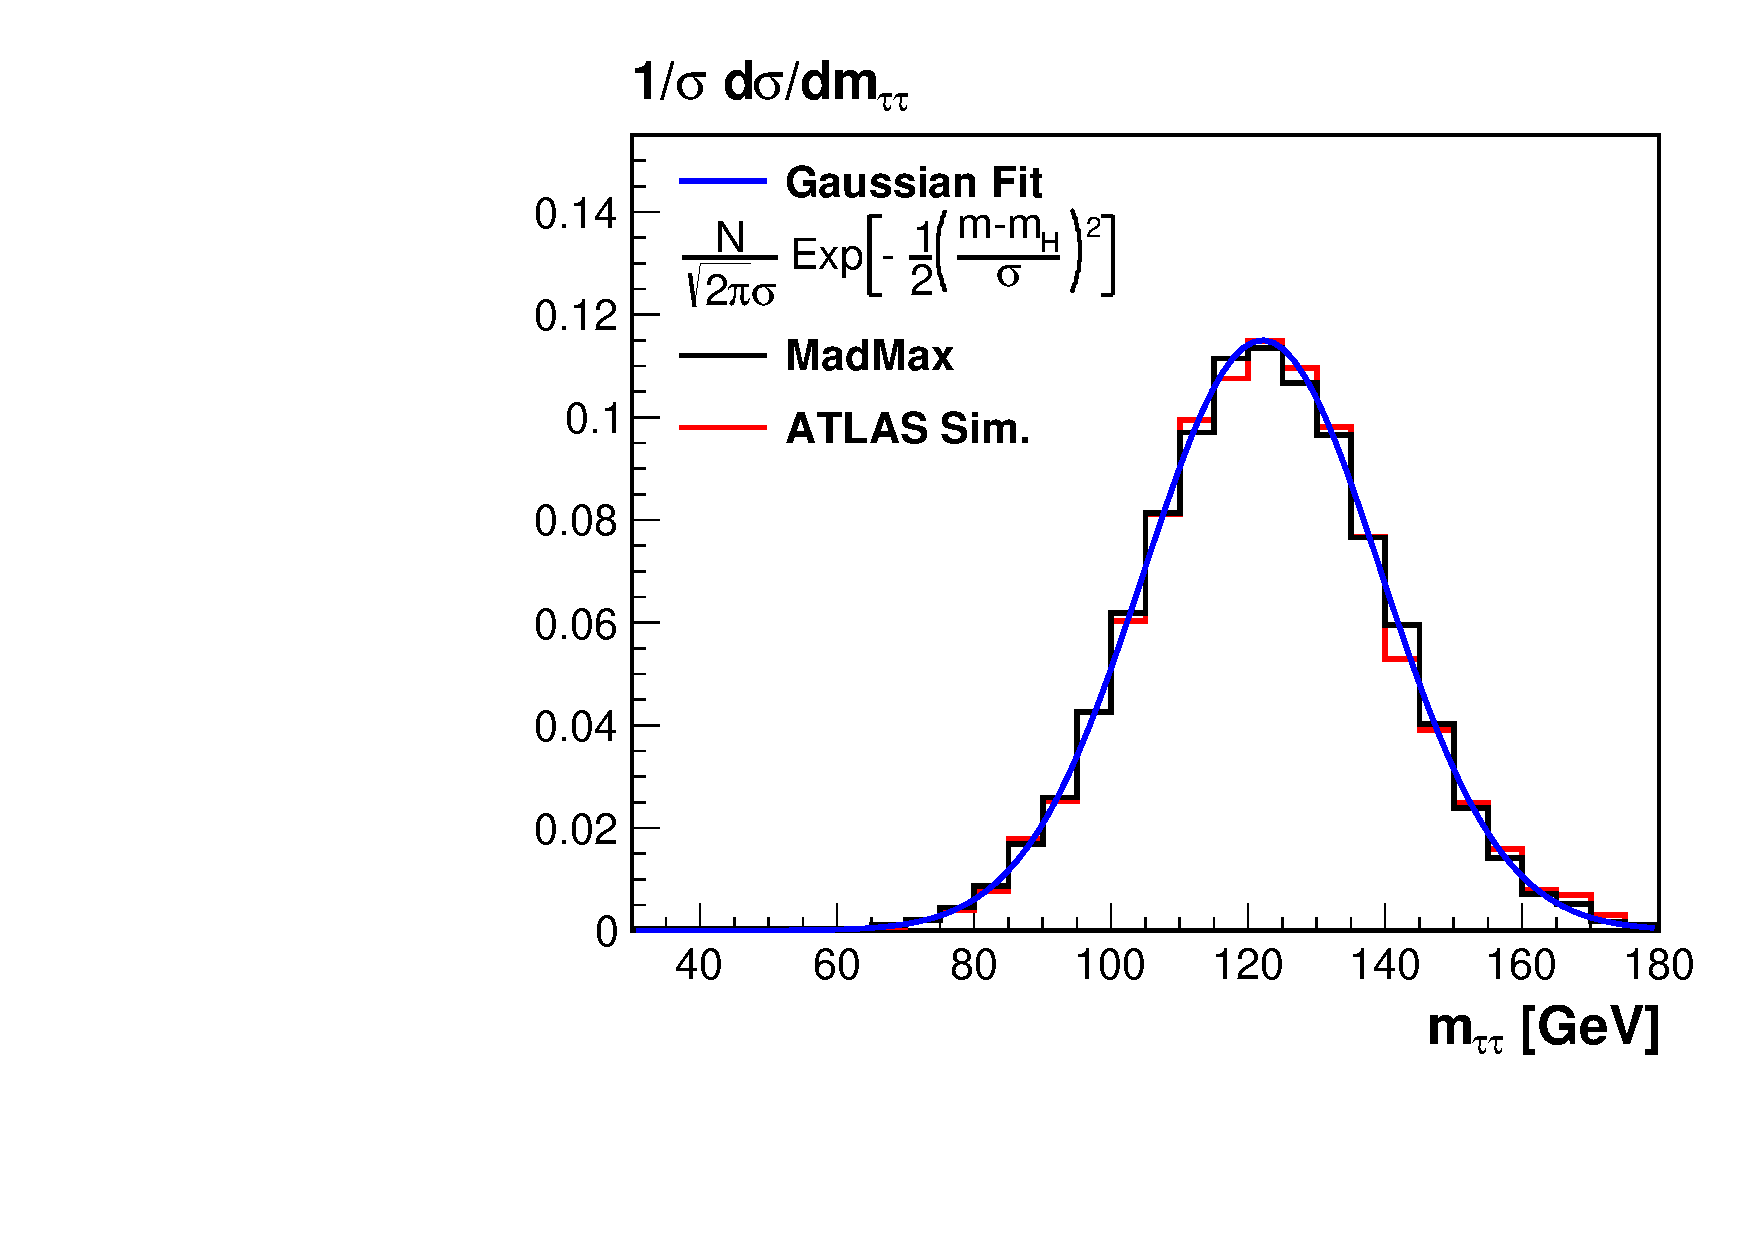
\includegraphics[width=0.49 \textwidth]{fig/information/wbf_tautau_smearing_mh}%
  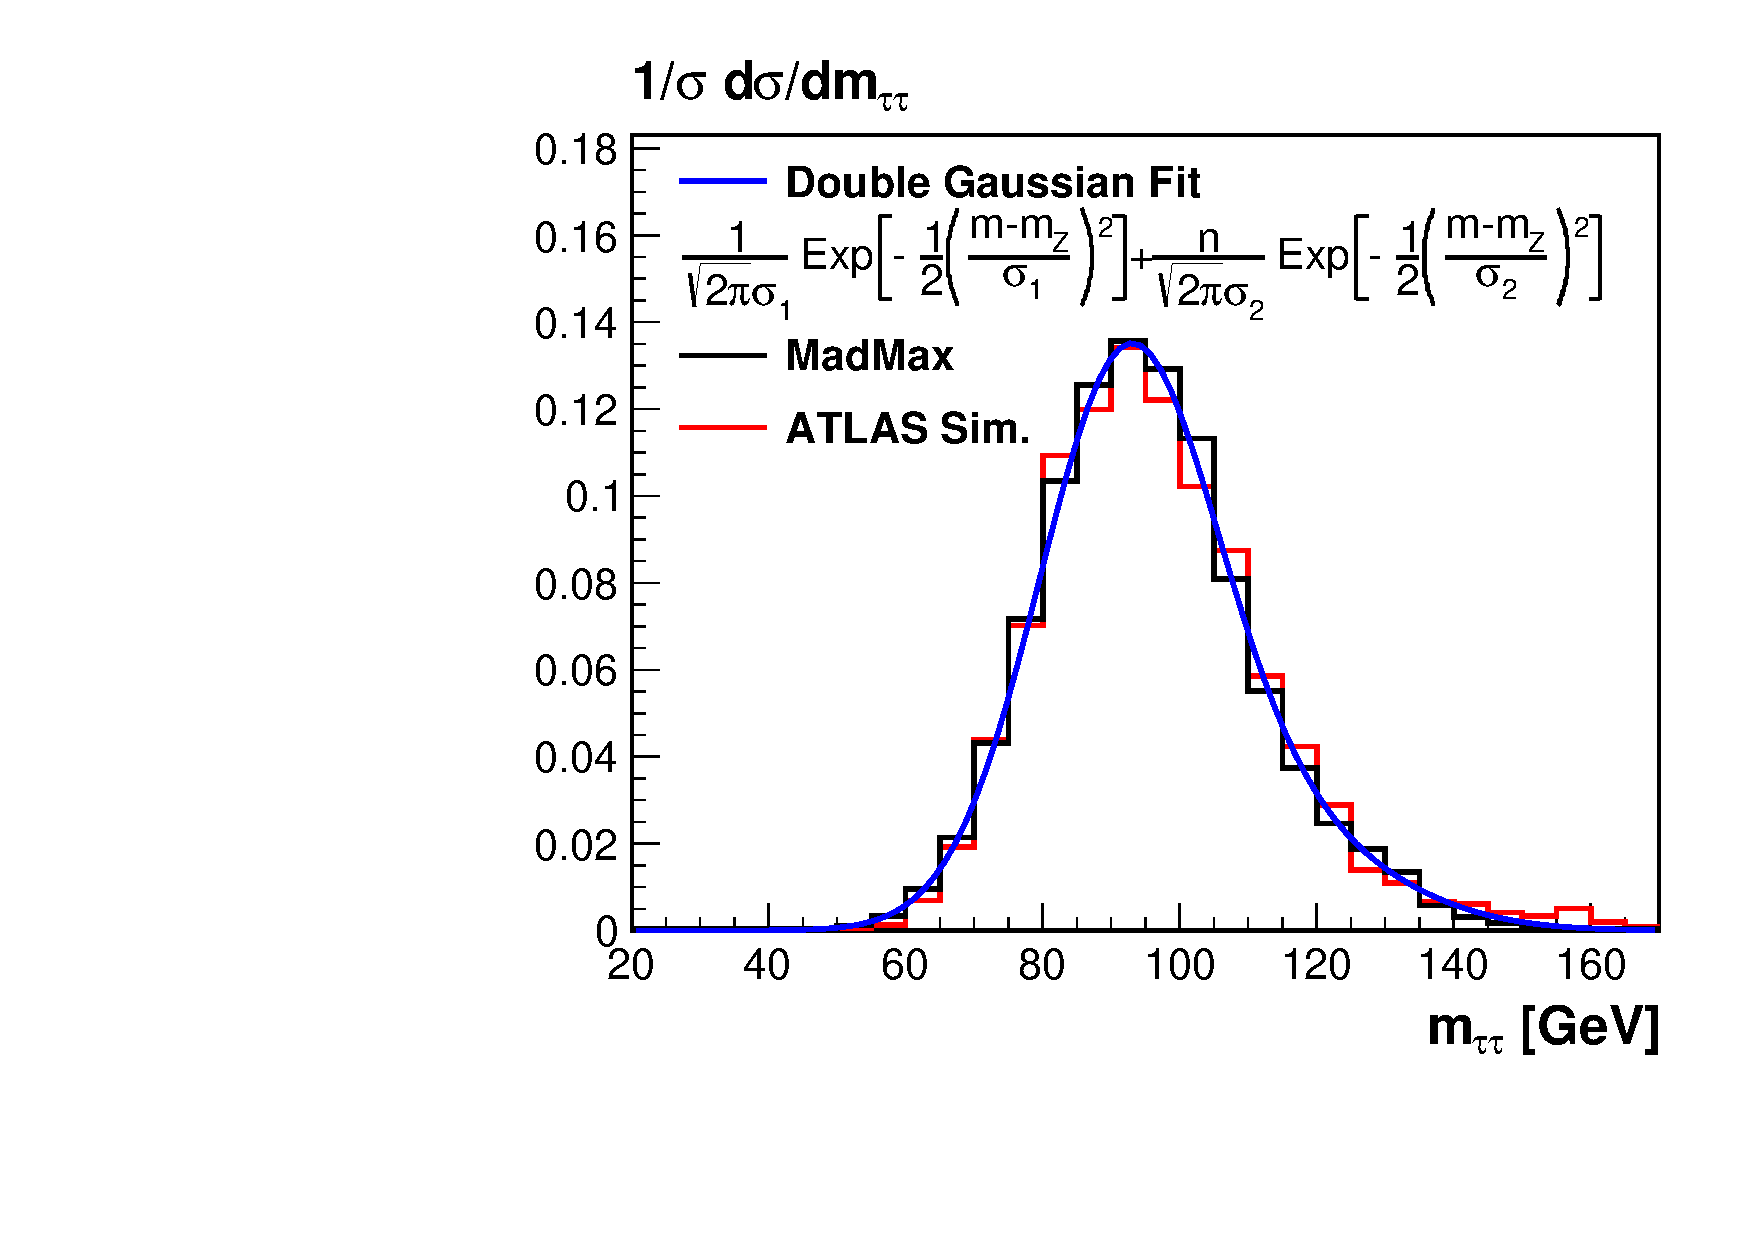
\includegraphics[width=0.49 \textwidth]{fig/information/wbf_tautau_smearing_mz}%
  \caption{Resolution effects in the invariant mass distribution in
    WBF Higgs production with $h \to \tau \tau$ for the Higgs
    contributions (left) and the $Zjj$ backgrounds (right). We show
    the ATLAS data from Reference~\cite{Aad:2015vsa} (black), the
    fitted response function (blue), and our final $\toolfont{MadMax}$
    output including the smearing function.}
  \label{fig:information_wbf_tautau_smearing}
\end{figure}

In the $4\ell$ channel, the backgrounds are negligible around
$m_{4\ell} \approx m_h$, so we do not have to include a smearing to
estimate the discrimination power. For Higgs production with a single
top in the $h \to \gamma \gamma$ mode, we follow
Reference~\cite{Kling:2016lay} and smear the $m_{\gamma \gamma}$
distribution of the signal process with a Gaussian of width
$1.52~\gev$. This resolution is based on Figure~6b of
Reference~\cite{CMS:2016zjv}.
%
% While this smearing function underestimates the signal contribution
% in the tails $m_{\gamma \gamma} \lesssim 120~\gev$ and
% $m_{\gamma \gamma} \gtrsim 130~\gev$, these phase-space regions do
% not carry a lot of information anyway.


%%%%%%%%%%%%%%%%%%%%%%%%%%%%%%%%%%%%%%%%%%%%%%%%%%%%%%%%%%%%
\subsection{Additional results}
\label{sec:appendix_information_additional_plots}
%%%%%%%%%%%%%%%%%%%%%%%%%%% %%%%%%%%%%%%%%%%%%%%%%%%%%%%%%%%%

\autoref{fig:information_wbf_tautau_grid} shows how the Fisher
information in the WBF $h \to \tau \tau$ channel changes with
$\boldtheta$.

\begin{figure}
  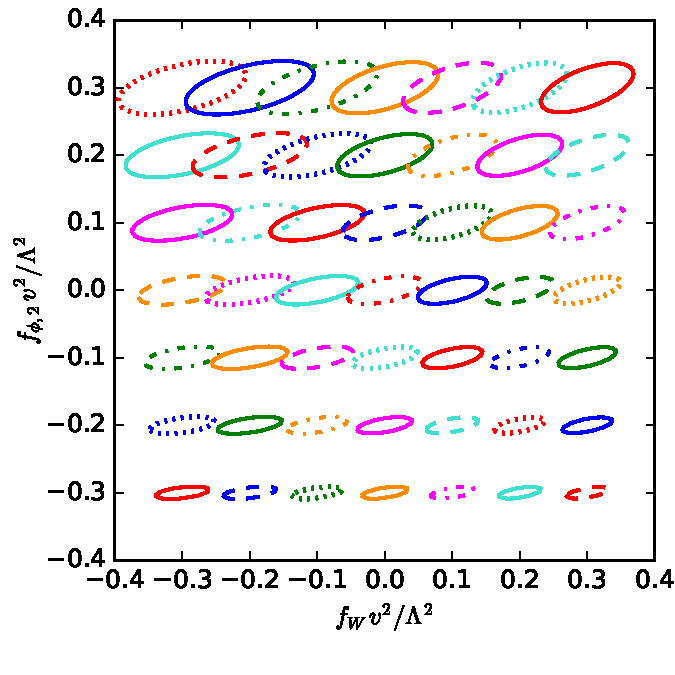
\includegraphics[width=0.33 \textwidth,clip,trim=0.3cm 0 0.05cm 0]{fig/information/wbf_tautau_grid_fphi2_fw}%
  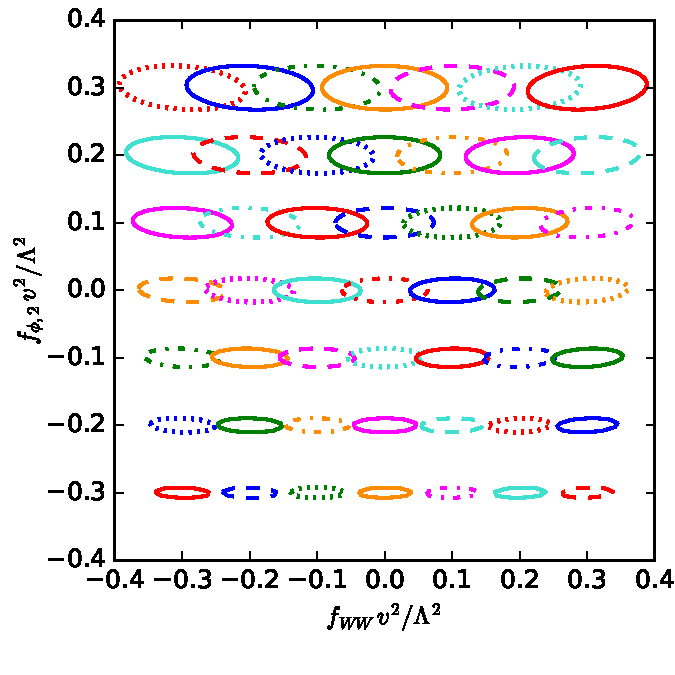
\includegraphics[width=0.33 \textwidth,clip,trim=0.3cm 0 0.05cm 0]{fig/information/wbf_tautau_grid_fphi2_fww}%
  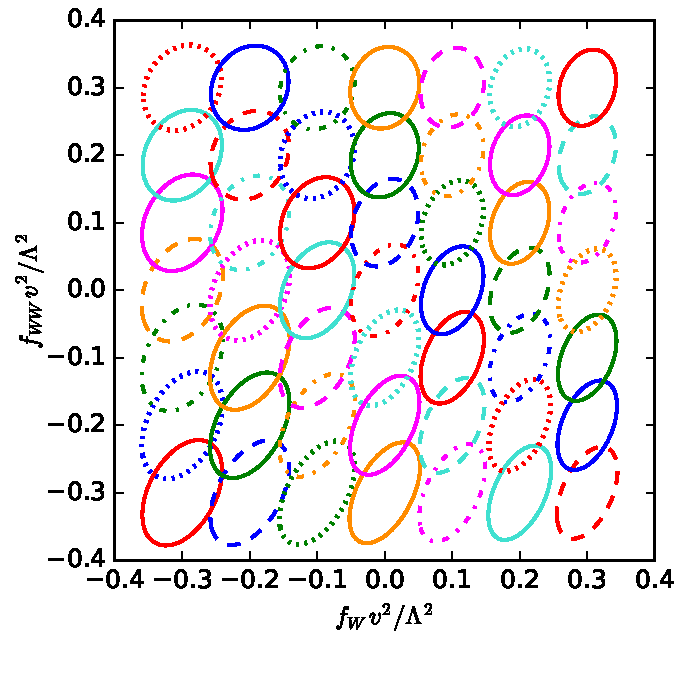
\includegraphics[width=0.33 \textwidth,clip,trim=0.3cm 0 0.05cm 0]{fig/information/wbf_tautau_grid_fww_fw}%
  \caption{Full Fisher information in the WBF $h \to \tau \tau$
    channel at different points in the parameter space. We visualise
    the Fisher information with contours of local distance
    $d_\text{local}(\boldtheta ; \boldtheta_0) = 1$, setting the
    $\theta_i$ not shown to zero. }
\label{fig:information_wbf_tautau_grid}
\end{figure}